\documentclass[10pt,twocolumn,twoside]{IEEEtran}
%\documentclass[10pt,onecolumn]{IEEEtran}
%\usepackage{setspace}
%\doublespacing
\usepackage{amsmath,amsopn,amssymb,stackrel}
\usepackage{graphicx,xspace,color,soul}
\usepackage{epsfig,subfigure}
\usepackage{longtable,multirow}
\usepackage{array,float}
\usepackage{cite,citesort}
\usepackage{url}
% make vector in bold
\renewcommand{\vec}[1]{\mathbf{#1}}
\usepackage{algorithm,algorithmicx,algpseudocode}
\renewcommand{\algorithmicrequire}{\textbf{Input:}}
\renewcommand{\algorithmicensure}{\textbf{Output:}}
\newcommand\floor[1]{\lfloor#1\rfloor}
\newcommand\ceil[1]{\lceil#1\rceil}

\usepackage{epstopdf}
\usepackage{stfloats}


\newcommand{\red}[1] {\textcolor[rgb]{1.0,0.0,0.0}{{#1}}}
\newcommand{\blue}[1] {\textcolor[rgb]{0.0,0.0,1.0}{{#1}}}

\newcounter{mytempeqncnt}
\graphicspath{{figs/}}

\begin{document}
\title{Joint Denoising / Compression of Image Contours via Shape Prior and Context Tree}

\author{
Amin Zheng~\IEEEmembership{Student Member,~IEEE},
Gene Cheung~\IEEEmembership{Senior Member,~IEEE},
Dinei Florencio~\IEEEmembership{Fellow,~IEEE}
\begin{small}
\thanks{A. Zheng is with 
        Department of Electronic and Computer Engineering, 
        The Hong Kong University of Science and Technology, 
        Clear Water Bay, Hong Kong, China
        (e-mail: amzheng@connect.ust.hk).}
        \thanks{G. Cheung is with 
        National Institute of Informatics, 2-1-2, Hitotsubashi, Chiyoda-ku,
        Tokyo, Japan 101--8430 
        (e-mail: cheung@nii.ac.jp).}
        \thanks{D. Florencio is with  
        Microsoft Research,
        Redmond, WA USA 
        (e-mail: dinei@microsoft.com).}
%Phone Number: +1-778-782-7159 Fax Number: +1-778-782-4951
\end{small}
}%
\maketitle
\vspace{0.1in}

\begin{abstract}
With the advent of depth sensing technologies, the extraction of object contours in images---a common and important pre-processing step for later higher-level computer vision tasks like object detection and human action recognition---has become easier. 
However, acquisition noise in captured depth images means that detected contours suffer from unavoidable errors. 
In this paper, we propose to jointly denoise and compress detected contours in an image for bandwidth-constrained transmission to a client, who can then carry out aforementioned application-specific tasks using the decoded contours as input.
We first prove theoretically that in general a joint denoising / compression approach can outperform a separate two-stage approach that first denoises then encodes contours lossily.
Adopting a joint approach, we first propose a burst error model that models typical errors encountered in an observed string $\vec{y}$ of directional edges.
We then formulate a rate-constrained maximum a posteriori (MAP) problem that trades off the posterior probability $P(\hat{\vec{x}} | \vec{y})$ of an estimated string $\hat{\vec{x}}$ given $\vec{y}$ with its code rate $R(\hat{\vec{x}})$. 
We design a dynamic programming (DP) algorithm that solves the posed problem optimally, and propose a compact context representation called total suffix tree (TST) that can reduce complexity of the algorithm dramatically.
Experimental results show that our joint denoising / compression scheme outperformed a competing separate scheme in rate-distortion performance noticeably.
\end{abstract}

\begin{IEEEkeywords}
contour coding, joint denoising / compression, image compression
\end{IEEEkeywords}

\IEEEpeerreviewmaketitle

%\vspace{-0.05in}
\section{Introduction}
\label{sec:intro}
Reinforcement learning has achieved great success in areas such as Game-playing \citep{silver2018general,vinyals2019grandmaster}, robotics \cite{kober2013reinforcement}, large language models \citep{ouyang2022training}, etc.
However, due to safety concerns or physical limitations, in some real-world reinforcement learning problems, we must consider additional constraints that may influence the optimal policy and the learning process \citep{garcia2015comprehensive}.
% For example, a robotic arm must not take actions that may cause harm to itself or the environments.
A standard framework to handle such cases is the constrained Markov Decision Process (CMDP) \citep{altman1999constrained}.
Within the CMDP framework, the agent has to maximize
the expected cumulative reward while
obeying a finite number of constraints, which are usually in the form of expected cumulative cost criteria.

However, we are sometimes concerned with the problem with a continuum of constraints.
For example,
the constraints we meet might be time-evolving or subject to uncertain parameters, which
cannot be formulated as an ordinary CMDP
(see Examples \ref{Example_Time_Evolving} and  \ref{Example_Uncertain}).
In this paper we would study a generalized CMDP  
to address the above problem.  Because the constraints are not only infinite-number but also lie
in a continuous set,
the generalization is not trivial. Fortunately, we find that we can borrow the idea behind semi-infinite programming (SIP) \citep{remez1934determination, hettich1993semi} to deal with the semi-infinite constraints.
Accordingly, we propose \emph{semi-infinitely constrained Markov decision processes} (SICMDPs)
as a novel complement to the ordinary CMDP framework.
%More specifically,  an SICMDP model %, we consider 
%contains a continuum of constraints whereas an ordinary CMDP contains a finite number of constraints. 

%This generalization is natural but not trivial. However, we can brows the idea  
%The idea is quite natural and can be backtracked
%to the practice of extending linear programming to linear semi-infinite programming (LSIP) %\cite{remez1934determination, GobernaLSIO1998}.
%In addition, 
%As a complementary approach to the ordinary CMDP framework, 
%SICMDP can be used to model these problems  which cannot be described by a finite number of constraints
%that are not covered by .
%For example,
%the restrictions we consider can be time-evolving or subject to uncertain parameters
%, thus
%cannot be described by a finite number of constraints but a continuum of constraints 
%(see Examples \ref{Example_Time_Evolving} and  \ref{Example_Uncertain}).

We also present two reinforcement learning algorithms to solve SICMDPs called SI-CRL and SI-CPO, respectively.
SI-CRL is a model-based reinforcement learning algorithm designed for tabular cases, and SI-CPO is a policy optimization algorithm for non-tabular cases.
% and analyze its performance both theoretically and empirically.
The main challenge is that we need to deal with a continuum of constraints, thus reinforcement learning algorithms for ordinary CMDPs do not work anymore.
In SI-CRL, we tackle this difficulty by first transforming the reinforcement learning problem to an equivalent LSIP problem, which can then be solved using methods in the LSIP literature like the dual exchange methods \citep{Hu1990,reemtsen1998numerical}.
In SI-CPO, we resort to the idea of cooperative stochastic approximation developed in \cite{lan2020algorithms, wei2020comirror}.
As far as we know, we are the first to introduce tools from semi-infinitely programming (SIP) into the reinforcement learning community for solving constrained reinforcement learning problems.

% To the best of our knowledge, we are the first to apply tools from semi-infinitely programming (SIP) to solve reinforcement learning problems.
Furthermore, we give theoretical analysis for both SI-CRL and SI-CPO.
We decompose the error of SI-CRL into two parts: the statistical error from approximating the true SICMDP with an offline dataset and the optimization error due to the fact that the solution of the LSIP problem obtained by the dual exchange method is inexact.
On the optimization side, we show that the iteration complexity of SI-CRL is $O\left(\left\{\mathrm{diam}(Y)L\sqrt{|\gS|^2|\gA|m}/\left[(1-\gamma)\epsilon\right]\right\}^m\right)$.
On the statistical side, we show that the sample complexity of SI-CRL is $\widetilde O\left(\frac{|S|^2|A|^2}{\epsilon^2(1-\gamma)^3}\right)$ if the offline dataset is generated by a generative model, and $\widetilde O\left(\frac{|S||A|}{\nu_{\min} \epsilon^2(1-\gamma)^3}\right)$ if the dataset is generated by a probability measure $\nu$ as considered in \cite{chen2019information}.
Here $\widetilde O$ means that all logarithm terms are discarded.
For SI-CPO, things become a little more complicated because other than the statistical error and the optimization error, we also need to consider the function approximation error, which comes from imperfect policy parametrizations.
It is shown if the function approximation error can be controlled to $O(\epsilon)$ order, the iteration complexity of SI-CPO is $\widetilde{O}\left(\frac{1}{\epsilon^2(1-\gamma)^6}\right)$ and the sample complexity of SI-CPO is $\widetilde{O}(\frac{1}{\epsilon^4(1-\gamma)^{10}})$.
Here our iteration complexity bound is equivalent to a typical $\widetilde O(1/\sqrt{T})$ global convergence rate.

We perform a set of numerical experiments to illustrate the SICMDP model and validate our proposed algorithms.
Specifically, we examine two numerical examples, namely the discharge of sewage and ship route planning.
Through the discharge of sewage example, we show the advantage of the SICMDP framework over the CMDP baseline obtained by naive discretization in modeling realistic sequential decision-making problems.
Moreover, we demonstrate the effectiveness of the SI-CRL and SI-CPO algorithms in such tabular environments. 
In the ship route planning example, we illustrate the benefits of the SICMDP framework and the ability of the SI-CPO algorithm to address complex continuous control tasks involving continuous state spaces with modern deep reinforcement learning techniques.

% In summary, our contributions are listed as follows.
% First, we present the SICMDP model, which can be viewed as a generalization of the ordinary CMDP model.
% Second, we propose an algorithm to perform reinforcement learning for SICMDPs, which is called SI-CRL, and we believe that we are the first to apply tools from SIP
% to solve reinforcement learning problems.
% Third, we give a theoretical analysis of SI-CRL and identify both its sample complexity and iteration complexity.
% In addition, we perform numerical experiments to illustrate the SICMDP model and validate the SI-CRL algorithm.
% \{This paragraph can be removed!!! \}






%\vspace{-0.1in}
\section{Related Work}
\label{sec:related}
\textbf{Related work}:
% Object detection related datasets/algo in non-medical domain
% Locally labeled CXR dataset
A few CXR datasets have localized abnormality annotations \cite{shih2019augmenting,filice2020crowdsourcing,jaeger2014two} that are curated manually. These are high quality gold standard ground truth datasets but tend to be smaller in scale (< 30,000 images) and have a narrow coverage, with typically only 1-2 labels. In addition, since most labeling efforts only have abnormality semantics attached, no direct relationships with the affected anatomical locations are available. 

%MEHDI: repeated concepts from above. I am removing the following: 

%The lack of anatomic semantics in the annotation is a limitation for complex multi-modal clinical reasoning work, e.g., differential diagnosis, since clinicians often integrate information along anatomical lines, and for downstream report generation tasks, which often requires describing not only the abnormality but also correctly communicate the location of the abnormalities (and medical devices) to the receiving clinicians. 

Two recent CXR datasets have labels for anatomies described in the reports. In \cite{datta2020dataset}, a small manually annotated dataset (2000 reports) included 10 abnormalities that are individually associated with 29 unique spatial locations (anatomies) at the report level. Another CXR dataset has automatically extracted abnormality and anatomy labels as disconnected concepts that are only correlated at the study level from  160,000 reports using a supervised NLP algorithm \cite{bustos2020padchest}. This was trained on a smaller set of manually annotated data. Neither datasets contain localized annotations for the associated CXR images, nor any comparison relation annotations between sequential exams, both of which are available in the Chest ImaGenome dataset. In Table \ref{tab:related}, we present a comparison of our Chest ImagGenome dataset with other datasets available in the literature.

% Table -- Kashyap

% MEdical imaging datasets to go here: Discussed that we will only focus on cxr datasets that are available for this paper. 
% \caption{\color{red} Kashyap, feel free to continue with the table. We should remove the questionmarks and add a line for our dataset (since all others are not graph). For longer text, using abbreviations and explaining them in the caption often works better. If fill in the values is not possible, it is better to remove the table altogether.}


\begin{table}[t!]
\caption{Summary of existing chest X-ray datasets}
\resizebox{\textwidth}{!}{%
\begin{tabular}{@{}lllllllll@{}}
\toprule
\textbf{Dataset} & \textbf{Annotation Level} & \textbf{Annotation Method} & \textbf{Num Labels} & \textbf{Anatomy Labeled} & \textbf{Graph} & \textbf{Dataset Size} & \textbf{Temporal Labels} & \textbf{Reports} \\ \midrule
SIIM-ACR Pneumothorax Segmentation \cite{filice2020crowdsourcing} & Segmentation & Manual + augmented & 1 & No & No & 12,047 & No & No \\
RSNA Pneumonia Detection Challenge   \cite{shih2019augmenting} & Bounding Boxes & Manual & 1 & No & No & 30,000 & No & No \\
Indiana University Chest X-ray collection \cite{demner2016preparing} & Global & Automated & 10 & No & No & 3,813 & No & Yes \\
NIH CXR dataset \cite{wang2017chestx} & Global & Automated & 14 & No & No & 112,120 & No & No \\
PLCO \cite{team2000prostate} & Global & Automated & 24 & Yes & No & 236,000 & Yes & No \\
Stanford CheXpert \cite{irvin2019chexpert} & Global & Automated & 14 & No & No & 224,316 & No & No \\
MIMIC-CXR \cite{johnson2019mimic} & Global & Automated & 14 & No & No & 377,110 & No & Yes \\
Dutta \cite{datta2020dataset} & Global & Manual & 10 & Yes & Yes & 2,000 & No & Yes \\
PadChest \cite{bustos2020padchest} & Global & Manual + automated & 297 & Yes & No & 160,868 & No & Yes \\
Montgomery County Chest X-ray   \cite{jaeger2014two} & Segmentation & Manual & 1 & Yes & No & 138 & No & No \\
Shenzen Hospital Chest X-ray   \cite{jaeger2014two} & Segmentation & Manual & 1 & Yes & No & 662 & No & No \\  \hline \hline
\textbf{Chest ImaGenome} & Bounding Boxes & Automated & 131 & Yes & Yes & 242,072 & Yes & Yes \\
\bottomrule
\end{tabular}%
}
\label{tab:related}
\vspace{-0.4cm}
\end{table}
% removed (Derived from MIMIC-CXR \cite{johnson2019mimic}) % makes table really small


%\vspace{-0.05in}
\section{Problem Formulation}
\label{sec:problem}
%!TEX root = main.tex
\section{Problem Definition and Notations}
\label{sec:problem}







% In this section, we will first describe key concepts and notations used in this paper, and formally define our problem. Then we will use a case study to make our idea of story tree more concrete.

% \subsection{Problem Definition and Notations}
% \label{subsec:problem-define}

We first present some definitions of key concepts in the top-down hierarchy: \textit{topic} $\rightarrow$ \textit{story} $\rightarrow$ \textit{event} to be used in this paper.

\begin{definition}
  \textit{Event}: an event $\mathcal{E}$ is a set of one or several documents that contain highly similar information.
\end{definition}

\begin{definition}
  \textit{Story}: a story $\mathcal{S}$ is a tree of events that revolve around a group of specific persons and happen at certain places during specific times. A directed edge from event $\mathcal{E}_1$ to $\mathcal{E}_2$ indicates a temporal evolution or a logical connection from $\mathcal{E}_1$ to $\mathcal{E}_2$.
\end{definition}

\begin{definition}
  \textit{Topic}: a topic consists of a set of stories that are highly correlated or similar to each other.
  \vspace{-1mm}
\end{definition}


Each topic may contain multiple story trees, and each story tree consists of multiple logically connected events.
In our work, events (instead of news documents) are the smallest atomic units. Each event is also assumed to belong to a single story and contains partial information about that story.
For instance, considering the topic \textit{American presidential election}, \textit{2016 U.S. presidential election} is a story within this topic, and  \textit{Trump and Hilary's first television debate} is an event within this story.


We now introduce some notations and describe our problem formally. Given a news document stream $D = \{ \mathcal{D}_1, \mathcal{D}_2, \ldots, \mathcal{D}_t,\ldots \}$, where $\mathcal{D}_t$ is the set of news documents collected on time period $t$, our objective is to: a) cluster all news documents $D$ into a set of events $E = \{ \mathcal{E}_1, \ldots, \mathcal{E}_{|E|} \}$, and b) connect the extracted events to form a set of stories $S = \{ \mathcal{S}_1, ..., \mathcal{S}_{|S|} \}$. Each story $\mathcal{S} = (E, L)$ contains a set of events $E$ and a set of links $L$, where $L_{i,j} := <\mathcal{E}_i, \mathcal{E}_j>$ denotes a directed link from event $\mathcal{E}_i$ to $\mathcal{E}_j$, which indicates a temporal evolution or logical connection relationship.

%We now illustrate our problem with an example. (A example Fig) Fig... shows ...
Furthermore, we require the events and story trees to be extracted in an online or incremental manner. That is, we extract events from each $\mathcal D_t$ individually when the news corpus $\mathcal D_t$ arrives in time period $t$, and \emph{merge} the discovered events into the existing story trees that were found at time $t-1$. This is a unique strength of our scheme as compared to prior work, since we do not need to repeatedly process older documents and can deliver  a set of evolving yet logically consistent story trees to users.  

% \subsection{Case Study}
% \label{subsec:case-study}

\begin{figure}
\includegraphics[width=3.4in]{figure/StoryStructures}
\caption{Different structures to characterize a story.}
\vspace{-2mm}
\label{fig:storyStructures}
\vspace{-2mm}
\end{figure}

For example, Fig.~\ref{fig:CaseStudy} illustrates the story tree of ``2016 U.S. presidential election''. The story contains $20$ nodes, where each node indicates an event in 2016 U.S. election, and each link indicates a temporal evolution or a logical connection between two events. %For example, event $19$ says America votes to elect new president, and event $20$ says Donald Trump is elected president. 
The index number on each node represents the event sequence over the timeline. There are $6$ paths within this story tree, where the path $1 \rightarrow 20$ indicates the whole presidential election process, branch $3 \rightarrow 6$ is about Hilary's health conditions, branch $7 \rightarrow 13$ talks about television debates, $14 \rightarrow 18$ depicts the investigation into Hilary's ``mail door'', etc. As we can see, by modeling the evolutionary and logical structure of a story into a story tree, users can easily grasp the logic of news stories and learn the main information quickly. 


Let us represent each story by an empty root node $s$ from which the story is originated, and denote each event by an event node $e$. The events in a story can be organized in one of the following four structures shown in Fig. \ref{fig:storyStructures}: a) a flat structure that does not include dependencies between events; b) a timeline structure that organizes events by their timestamps; c) a graph structure that checks the connection between all pairs of events and maintains a subset of most strong connections; d) a tree structure, which represents a story's evolving structure by a tree.  

Compared with a tree structure, sorting events by timestamps omits the logical connection between events, while using directed acyclic graphs to model event dependencies without considering the evolving consistency of the whole story can leads to unnecessary connections between events.
Through extensive user experience studies in Sec.~\ref{sec:eval}, we show that tree structures are the most effective way to represent breaking news stories as compared to other structures, including the more complex graph structures. 


%\vspace{-0.05in}
\section{Error Term}
\label{sec:error}
\documentclass[a4paper,twoside]{article}      % Comments }      % Comments after  % are ignored
\usepackage{amsmath,amssymb,amsfonts,amsthm,amscd}
%\usepackage{graphics}
\usepackage{graphicx}
\usepackage{a4wide}
\usepackage{enumerate}
\usepackage{color}
\usepackage{mathrsfs}
\usepackage{authblk}
\def\R{\mathbb{R}}
\newtheorem{theorem}{Theorem}[section]
\newtheorem{proposition}[theorem]{Proposition}
\newtheorem{corollary}[theorem]{Corollary}
\newtheorem{lemma}[theorem]{Lemma}
\newtheorem{conjecture}[theorem]{Conjecture}
\theoremstyle{definition}
\newtheorem{remark}[theorem]{Remark}
\newtheorem{algorithm}[theorem]{Algorithm}
\def\H{\bar{H}}
\def\P{\bar{P}}
\def\Q{\bar{Q}}
\def\F{\bar{F}}
\def\f{\bar{f}}
\def\h{\bar{h}}
\def\kb{\bar{k}}
\def\N{\mathcal{N}}
\def\ph{\hat{p}}
\def\ah{\hat{a}}
\def\bh{\hat{b}}
\def\Ph{\hat{P}}
\def\ph{\bar{h}}
\def\bm{\bar{m}}
\def\bs{\bar{\sigma}}
\def\L{\mathscr{L}}
\def\cL{\mathcal{L}}
\def\A{\mathscr{A}}
\def\E{\mathcal{E}}
\def\H{\mathcal{H}}
\def\V{\mathcal{V}}
\def\C{\mathcal{C}}
\def\B{\mathcal{B}}
\def\Em{E^{\mathrm{mix}}}
\def\div{\mathop{\mathrm{div}}\nolimits}
\let\endremark\qed
\newtheorem{definition}[theorem]{Definition}
\newtheorem{example}{Example}[section]
\newtheorem{assumption}{Assumption}[section]
\newtheorem{question}{Question}[section]
\usepackage{hyperref}
%\mathtoolsset{showonlyrefs}
\hypersetup{
    bookmarks=true,         % show bookmarks bar?
    unicode=false,          % non-Latin characters in Acrobat‚????s bookmarks
    pdftoolbar=true,        % show Acrobat‚????s toolbar?
    pdfmenubar=true,        % show Acrobat‚????s menu?
    pdffitwindow=false,     % window fit to page when opened
    pdfstartview={FitH},    % fits the width of the page to the window
    pdftitle={My title},    % title
    pdfauthor={Author},     % author
    pdfsubject={Subject},   % subject of the document
    pdfcreator={Creator},   % creator of the document
    pdfproducer={Producer}, % producer of the document
    pdfkeywords={keywords}, % list of keywords
    pdfnewwindow=true,      % links in new window
    colorlinks=true,       % false: boxed links; true: colored links
    linkcolor=blue,          % color of internal links
    citecolor=blue,        % color of links to bibliography
    filecolor=magenta,      % color of file links
    urlcolor=cyan           % color of external links
}
\newcommand{\ty}{\textcolor{yellow}}
\newcommand{\tr}{\textcolor{red}}
\newcommand{\tb}{\textcolor{black}}
\newcommand{\AM}{\textcolor{black}}
\newcommand{\tg}{\textcolor[rgb]{0.60,0.20,0.80}}
\def\w{\omega}
\def\hg{\hat{\gamma}}

\title{Model reduction of Brownian oscillators: quantification of errors and long-time behaviour}
\author[1]{Matteo Colangeli\thanks{matteo.colangeli1@univaq.it}}
\author[2]{Manh Hong Duong\thanks{h.duong@bham.ac.uk}}
\author[3]{Adrian Muntean\thanks{adrian.muntean@kau.se}}
\affil[1]{Department of Information Engineering, Computer Science and Mathematics,
University of L'Aquila, Italy.}
\affil[2]{School of Mathematics,
University of Birmingham,
UK.}
\affil[3]{Department of Mathematics and Computer Science \& Centre for Societal Risk Research (CSR), Karlstad University, Sweden.}

\begin{document}
\maketitle
\begin{abstract}
A procedure for model reduction of stochastic ordinary differential equations with additive noise was recently introduced in \cite{CDM22}, based on the Invariant Manifold method and on the Fluctuation-Dissipation relation. A general question thus arises as to whether one can rigorously quantify the error entailed by the use of the reduced dynamics in place of the original one. In this work we provide explicit formulae and estimates of the error in terms of the Wasserstein distance, both in the presence or in the absence of a sharp time-scale separation between the variables to be retained or eliminated from the description, as well as in the long-time behaviour.  

\AM{{\bf Keywords:} Model reduction, Wasserstein distance, error estimates, coupled Brownian oscillators, invariant manifold, Fluctuation-Dissipation relation.}
\end{abstract}
%\tableofcontents
\section{Introduction}
\label{sec:sec1}

The notion of scale separation is largely invoked in multiscale modelling and homogeneization methods \AM{(including model reduction and operator splitting techniques)} \cite{givon2004extracting,pavliotis2008multiscale}, and has also found far-reaching applications in different areas of science \AM{and engineering}, \textit{e.g.} in climate dynamics \cite{Ghil20},  biochemical systems \cite{Schnell17}, chemical reaction networks \cite{Kang2013}, \AM{smoldering combustion \cite{Ijioma2014}, and so on}. %\textcolor{red}{other possible fields of applications??}. 
A neat illustration of this \AM{notion} can be traced
in the preface of Haken's seminal book on Synergetics \cite{Haken2004}, where the author writes: ``In large classes of systems that are originally described by \textit{many} variables, the behavior of a system is described and determined by only \textit{few} variables, the \textit{order parameters}. They fix the behavior of the individual parts via the \textit{slaving principle}''. A physical rationale behind the slaving principle amounts to the assumption of decomposition of motions: there exists a short time-scale during which the slow variable does not change significantly, while the fast variable rapidly settles on a value determined by the slow one. The evolution of the latter, in turn, takes place on a much longer scale. 
A specific form of such principle is realized through the method of adiabatic elimination of fast variables, which underlies the derivation of the Smoluchowski equation from the underdamped Langevin equation. A sharp distinction between slow and fast variables is also a prerequisite for application of the Mori-Zwanzing method \cite{Zwanzig} in the derivation of reduced equations from higher dimensional stochastic dynamics, where the Markovian structure of the original process is preserved in the reduced description by stipulating a perfect time-scale separation.
The same guiding principle underpins, in kinetic theory, the Grad moment method \cite{Grad49,colan07b},  and has also been exploited in the derivation of linear hydrodynamics from the Boltzmann equation using the framework of the Invariant Manifold \cite{GorKar05,colan09}. 
The latter method has also been exploited in \cite{CDM22} to characterize the deterministic component of the contracted description in a system of two coupled (underdamped) Brownian harmonic oscillators. The structure of the noise term of the Markovian reduced dynamics, in turn, was determined via the Fluctuation-Dissipation relation. A general question, then, concerns the derivation of a quantitative estimate of the error stemming from the use of the reduced dynamics in place of the original one.
A first attempt, in this direction, was proposed in \cite{CM22}, and it was based on the study of the equilibrium correlation functions in the reduced and in the original processes. A uniform-in-time type of convergence of the correlations evaluated in the two processes was proven to hold in the so-called overdamped limit, where the friction parameter diverges.

In this work we take a step further, and compute explicitly the Wasserstein distance between the laws of the original and reduced processes. This paves the way to explicitly quantify the error inherent to the contracted description.
We focus on two classical models thoroughly studied in statistical physics and molecular dynamics, namely the underdamped Brownian harmonic oscillator and a system of two coupled overdamped Brownian harmonic oscillators. In the more traditional approach based on the slow-fast decomposition of motions, a reduced description can be achieved by passing the parameter to a certain limit, thus establishing a perfect time-scale separation, see e.g. \cite{Zwanzig,Ghil}. In the present work, instead, we derive the reduced dynamics in a regime characterized by a finite time-scale separation, which is controlled, in the two considered models, by either the friction parameter or the coupling parameter. We show that the reduced and original dynamics are exponentially close at any time, and they coincide if we pass the parameter to the corresponding limit. We also prove that the two dynamics have the same equilibrium measure and, furthermore, they exponentially converge to the equilibrium measure with the same rate. This notable property is a direct consequence of the proposed reduction scheme, in particular of the selection of solutions to the invariance equation obtained from the Invariant Manifold method. As a consequence of this, the spectrum of the reduced drift matrix is a subset of the spectrum of the original drift matrix. The models and precise statements of the results are presented in Section \ref{sec:sec3} and Section \ref{sec:sec4}.

The work is structured as follows. In Sec. \ref{sec:sec2} we review the definition of the Wasserstein distance between two probability measures and introduce the basic notation used throughout the manuscript. In Sec. \ref{sec:sec3} we compute our error estimate based on the Wasserstein distance for a Brownian harmonic oscillator, for which the laws of the original and the contracted descriptions are analytically known. In Sec. \ref{sec:sec4} we apply our method to a slightly more involved model, constituted by a pair of coupled overdamped Brownian harmonic oscillators. Conclusions and a final outlook are finally drawn in Sec. \ref{sec:sec5}.


\section{Preliminaries}
\label{sec:sec2}

In this Section we introduce the Wasserstein distance between two probability measures and also fix the notation used \AM{throughout} the manuscript.

\subsection{Wasserstein distance}
In this section we recall the definition of the Wasserstein distance between two probability measures and its explicit formula when the two probability measures are Gaussian distributions. The Wasserstein metric plays an central role in many research fields such as optimal transport, partial differential equations and data science. For a detailed account of the topics, we refer the reader to Villani's monograph \cite{Villani2003}.

Let $P_2(\R^d)$ be the space of probability measures $\mu$ on $\R^d$ with finite second moment, namely
$$
\int_{\R^d}|x|^2\mu(dx)<\infty.
$$
Let $\mu$ and $\nu$ be two probability measures belonging to $P_2(\R^d)$. The $L^2$-Wasserstein distance, $W_2(\mu,\nu)$, between $\mu$ and $\nu$ is defined via
\begin{equation}
\label{eq: W2}
W^2_2(\mu,\nu):=\inf_{\gamma\in \Gamma(\mu,\nu)}\int_{\R^d\times\R^d}|x-y|^2\,\gamma(dx,dy),
\end{equation}
where $\Gamma(\mu,\nu)$ denotes the set of all couplings between $\mu$ and $\nu$, i.e., the set of all probability measures on $\R^d\times \R^d$ having $\mu$ and $\nu$ as the first and the second marginals respectively. More precisely,
$$
\Gamma(\mu,\nu):=\{\gamma\in P(\R^d\times \R^d): \gamma(A\times \R^d)=\mu(A)~\text{and}~ \gamma(\R^d\times A)=\nu(A)\},
$$
for all Borel measurable sets $A\subset\R^d$. 



In particular, the Wasserstein distance between two Gaussian measures can be computed explicitly in terms of the means and covariance matrices  \cite{GivensShortt1984}, see also e.g., \cite{Takatsu2012}
\begin{equation}
\label{eq: W2-Gaussians}
W_2(\N(u,U),\N(v,V))^2=|u-v|^2+\mathrm{tr}U+\mathrm{tr}V-2\mathrm{tr}\sqrt{V^\frac{1}{2}U V^\frac{1}{2}},
\end{equation}
where $u, v$ are the means and $U, V$ are the covariance matrices.
In a one dimensional space, the above formula reduces to
\begin{equation}
W_2(\N(u_1,\sigma_1^2),\N(u_2,\sigma_2^2)^2=(u_1-u_2)^2+(\sigma_1-\sigma_2)^2.
\end{equation}
\subsection{Linear drift-diffusion equations}
\label{sec: linear SDE}
We recall here a well-known result \AM{concerning} the explicit solution of a general linear drift-diffusion where the initial data is a Gaussian distribution. In the subsequent sections, we will apply this result to our models of (coupled) Brownian oscillators.

\AM{To set the stage, we }consider the following general linear drift-diffusion equation
\begin{equation}
\label{eq: linear diffusion}
    \partial_t\rho=-\div(Cx\rho)+\div(D\nabla\rho),\quad \rho(0)=\rho_0.
\end{equation}
In the above equation, the unknown is a probability measure  $\rho=\rho(t,x)$ with $(t,x)\in (0,\infty)\times \mathbb{R}^d$; $C$ and $D$ are two constant matrices of order $d$ representing the drift and diffusion matrices; the initial data $\rho_0$ is a probability measure on $\mathbb{R}^d$.

The following lemma provides the explicit formula for the solution of \eqref{eq: linear diffusion} when the initial data is a Gaussian distribution, see for instance \cite{gomes2018mean}.
\begin{lemma}
\label{lem: Gaussian sol}
Suppose the initial data is a Gaussian, $\rho_0\sim \mathcal{N}(\mu(0),\Sigma(0))$, then the solution to \eqref{eq: linear diffusion} is given by 
\begin{equation}
\label{eq: MKEGaussian}
\rho(t,x)=\frac{1}{\sqrt{(2\pi)^d\det\Sigma(t)}}\exp\Big[-\frac{1}{2}(x-\mu(t))^T \Sigma^{-1}(t)(x-\mu(t))\Big]  
\end{equation}
where $\mu(t)$ and $\Sigma(t)$ are given by
\begin{equation}
\label{eq: MKE Gaussian mean-variance}
\mu(t):=e^{tC}\mu(0),\quad \Sigma(t):=e^{t C}\Sigma(0)e^{t C^T}+2\int_0^t e^{s C}De^{s C^T}\,ds.
\end{equation}
Under suitable conditions on $C$ and $K$, we have $\mu(t)\rightarrow 0$ and $\Sigma(t)\rightarrow \Sigma_\infty$ where
$$
\Sigma_\infty:=2\int_0^\infty e^{sC}De^{sC^T}\,ds.
$$
Note that $\Sigma_\infty$ satisfies the so-called Lyapunov equation
$$
2D=C\Sigma_\infty+\Sigma_\infty C^T.
$$
\end{lemma}
\subsection{Exponential of a $2\times 2$ matrix}
Lemma \ref{lem: Gaussian sol} provides \AM{the explicit form of the unique} solution to the linear drift-diffusion equation \eqref{eq: linear diffusion} when the initial data is a Gaussian. However, in general the formula \eqref{eq: MKE Gaussian mean-variance} is analytically hard to compute since it involves exponential of matrices. The following lemma provides an explicit formula for the exponential of a $2\times 2$ matrix, which will be used in the subsequent analysis.
\begin{lemma}
\label{lem: exponential matrix}
\AM{Let $a,b,c,d \in\mathbb{R}$ be taken arbitrarily with $a^2+b^2+c^2+d^2>0$.} The following identity holds
\begin{equation}\label{magic}
    \exp\begin{pmatrix}
        a&b\\c &d
    \end{pmatrix}=\frac{1}{\Delta}\begin{pmatrix}
        m_{11}&m_{12}\\
        m_{21}& m_{22}
    \end{pmatrix},
\end{equation}
where $\Delta:=\sqrt{(a-d)^2+4bc}$ and
\begin{align*}
    m_{11}&:=e^{(a+d)/2}\Big[\Delta \cosh{\frac{1}{2}\Delta} +(a-d)\sinh{\frac{1}{2}\Delta}\Big],\\
    m_{12}&:=2be^{(a+d)/2}\sinh{\frac{1}{2}\Delta},
    \\ m_{21}&:=2 c e^{(a+d)/2}\sinh{\frac{1}{2}\Delta},
    \\ m_{22}&:=e^{(a+d)/2}\Big[\Delta \cosh{\frac{1}{2}\Delta} +(d-a)\sinh{\frac{1}{2}\Delta}\Big].
\end{align*}
\end{lemma}

\begin{proof}\AM{We refer the reader to \cite{bernstein1993} for a justification of the formula \eqref{magic}.}
\end{proof}



\section{Model reduction of a Brownian oscillator}
\label{sec:sec3}

\AM{To start off the discussion, we begin with the investigation of a } simple model of an underdamped Brownian oscillator considered in \cite{CM22}, which is amenable to an explicit analytical solution.
The original dynamics reads as follows:
\begin{align*}
dx(t)&=v(t)\,dt\\
d v(t)&=-\omega^2 x(t)\,dt-\gamma v(t)\,dt+\sqrt{2\gamma\beta^{-1}}\,dW(t),\\
(x(0),v(0))&=(x_0,v_0)
\end{align*}
Exploiting the Invariant Manifold method and the Fluctuation-Dissipation relation (for a short summary of the method, see Section \ref{sec:sec4} below, where the same reduction procedure is applied to a system of coupled overdamped Brownian harmonic oscillators), the reduced dynamics attains the form: 
$$
d \bar{x}(t)=-\alpha \bar{x}(t)\,dt+\sqrt{2 D_r}\,dW(t),\quad \bar{x}(0)=x_0 ,
$$
where 
$$
\alpha=\frac{\gamma-\sqrt{\gamma^2-4\omega^2}}{2},\quad D_r=\frac{\alpha}{\omega^2\beta}.
$$ \AM{The reader is referred to \cite{CM22} to see the details of the calculations}. 
The main result of this section is the following theorem.
\begin{theorem} %The following statements hold true:
\begin{enumerate}[(i)]\
\item (exact solutions of the original and the reduced dynamics) $\mu_t$ and $\bar{\mu}_t$ are Gaussian measures 
\begin{equation}
\mu_t=\mathcal{N}(m(t),\sigma(t)),\quad \bar{\mu}_t=\mathcal{N}(\bar{m}_t,\bar{\sigma}(t)),
\end{equation}
where
\begin{align*}
m(t)&=\frac{\lambda_1 e^{-\lambda_2 t}-\lambda_2 e^{-\lambda_1 t}}{\lambda_1-\lambda_2}x_0+\frac{e^{-\lambda_2 t}-e^{-\lambda_1 t}}{\lambda_1-\lambda_2}v_0,\\
\sigma(t)&=\frac{\gamma \beta^{-1}}{(\lambda_1-\lambda_2)^2}\Big[\frac{\lambda_1+\lambda_2}{\lambda_1\lambda_2}+\frac{4}{\lambda_1+\lambda_2}(e^{-(\lambda_1+\lambda_2)t}-1)-\frac{1}{\lambda_1}e^{-2\lambda_1 t}-\frac{1}{\lambda_2}e^{-2\lambda_2 t}\Big],\\
\bar{m}(t)&=e^{-\lambda_2 t}\bar{x}_0,\\
\bar{\sigma}(t)&=\frac{1}{\omega^2 \beta}(1-e^{-2\lambda_2 t})
\end{align*}
where
\begin{equation}
\lambda_1=\frac{\gamma+\sqrt{\gamma^2-4\omega^2}}{2},\quad \lambda_2=\frac{\gamma-\sqrt{\gamma^2-4\omega^2}}{2}=\frac{2\omega^2}{\gamma+\sqrt{\gamma^2-4\omega^2}}.
\end{equation}
\item (Exact Wasserstein distance between the laws of the original and reduced dynamics) The Wasserstein distance between $\mu_t$ and $\bar{\mu}_t$ can be computed explicitly via
\begin{equation}
W_2^2(\mu_t,\bar{\mu}_t)=(m(t)-\bar{m}(t))^2+\Big(\sqrt{\sigma_{xx}(t)}-\sqrt{\bar{\sigma}(t)}\Big)^2.
\end{equation}
\item (explicit rate of convergence in the high-friction limit) It holds that
\begin{equation}
\label{eq: high-friction}
W_2^2(\mu_t,\bar{\mu}_t)\leq \frac{4}{\gamma^2-4\omega^2}\Big[(\omega |x_0|+|v_0|)^2+\frac{4}{\beta}\Big]\quad\forall t>0.
\end{equation}
As a consequence,
$$
\lim_{\gamma\rightarrow +\infty}W_2^2(\mu_t,\bar{\mu}_t)=0.
$$
Note that \eqref{eq: high-friction} is a much stronger statement providing an explicit rate of convergence.
\item (Common rates of convergence to equilibrium) There exists a constant $C>0$, which can be found explicitly, such that
$$
W_2(\mu_t,\mu_\infty),~ W_2(\bar{\mu}_t,\bar{\mu}_\infty)\leq C e^{-\lambda_2 t},
$$
where 
$$
\mu_\infty=\bar{\mu}_\infty=\mathcal{N}\Big(0, \frac{1}{\beta\omega^2}\Big).
$$
This result shows that the original dynamics and the reduced one not only share the same equilibrium, they have the same rates of convergence to equilibrium in the Wasserstein distance.
\item (long-time behaviour) It holds that
\begin{equation}
\label{eq: longtime}
W_2^2(\mu_t,\bar{\mu}_t)\leq \Big[\frac{\omega|x_0|+|v_0|}{\sqrt{\gamma^2-4\omega^2}}+\frac{10}{\beta(\gamma^2-4\omega^2)}\Big]e^{-\lambda_2 t}.
\end{equation}
As a consequence of this, we also have
$$
\lim_{t\rightarrow +\infty}W_2(\mu_t,\bar{\mu}_t)=0,
$$
which is already obtained in the previous part. Estimate \eqref{eq: longtime} is a stronger statement, showing that the two dynamics are exponentially close at any time $t>0$.
\item Suppose that the initial data $x_0$ is randomly distributed according to an even probability measure $\rho_0\in L^1(\mathbb{R})$ then the estimates in parts $(iii)$ and $(iv)$ still hold true.
\end{enumerate}
\end{theorem}
\begin{proof}\
$(i)$. The law $\rho_t$ of $z(t)=\begin{pmatrix}x(t)\\v(t)\end{pmatrix}$ satisfies the kinetic Fokker Planck equation
$$
\partial_t\rho_t=\mathscr{L}^*\rho_t, \quad \rho\vert_{t=0}=\delta_{(x_0,v_0)},
$$
where $\mathscr{L}^*\rho:=-v\partial_x\rho+\omega^2 x\partial_v\rho+\gamma \big[\partial_{v}(v \rho)+\beta^{-1}\partial^2_{vv}\rho\big]$.

According to [Risken, Section 10.2] $\mu_t$ is a bivariate Gaussian measure with mean $M(t)\in \mathbb{R}^2$ and covariane matrix $\Sigma(t)\in\mathbb{R}^{2\times 2}$. \AM{They are $t$ dependent objects} given by
$$
M(t)=\begin{pmatrix}
m_x(x)\\ m_v(t)
\end{pmatrix}, \quad \Sigma^{-1}(t)=\begin{pmatrix}
[\sigma_{xx}(t)]^{-1}&[\sigma_{xv}(t)]^{-1}\\
[\sigma_{vx}(t)]^{-1}&[\sigma_{vv}(t)]^{-1}
\end{pmatrix},
$$
where 
\begin{align*}
m_x(t)&=\frac{\lambda_1 e^{-\lambda_2 t}-\lambda_2 e^{-\lambda_1 t}}{\lambda_1-\lambda_2}x_0+\frac{e^{-\lambda_2 t}-e^{-\lambda_1 t}}{\lambda_1-\lambda_2}v_0,\\
m_v(t)&=\omega^2 \frac{e^{-\lambda_1 t}-e^{-\lambda_2 t}}{\lambda_1-\lambda_2} x_0+\frac{\lambda_1 e^{-\lambda_1 t}-\lambda_2 e^{-\lambda_2 t}}{\lambda_1-\lambda_2}v_0,\\
\sigma_{xx}(t)&=\frac{\gamma \beta^{-1}}{(\lambda_1-\lambda_2)^2}\Big[\frac{\lambda_1+\lambda_2}{\lambda_1\lambda_2}+\frac{4}{\lambda_1+\lambda_2}(e^{-(\lambda_1+\lambda_2)t}-1)-\frac{1}{\lambda_1}e^{-2\lambda_1 t}-\frac{1}{\lambda_2}e^{-2\lambda_2 t}\Big],\\
\sigma_{xv}(t)&=\frac{\gamma \beta^{-1}}{(\lambda_1-\lambda_2)^2}(e^{-\lambda_1 t}-e^{-\lambda_2 t})^2,\\
\sigma_{vv}(t)&=\frac{\gamma \beta^{-1}}{(\lambda_1-\lambda_2)^2}\Big[\lambda_1+\lambda_2+\frac{4\lambda_1\lambda_2}{\lambda_1+\lambda_2}(e^{-(\lambda_1+\lambda_2)t}-1)-\lambda	_1 e^{-2\lambda_1 t}-\lambda_2 e^{-2\lambda_2 t}\Big],
\end{align*} 
where
\begin{equation}
\label{eq: lambdas}
\lambda_{1}=\frac{\gamma+\sqrt{\gamma^2-4\omega^2}}{2},\quad \lambda_{2}=\frac{\gamma-\sqrt{\gamma^2-4\omega^2}}{2},\quad\text{thus}\quad \lambda_1+\lambda_2=\gamma,\quad \lambda_1\lambda_2=\omega^2,\quad \lambda_1-\lambda_2=\sqrt{\gamma^2-4\omega^2}.
\end{equation}
Note that, since in the overdamped regime $\gamma\geq 2\omega$, we have
$$
\lambda_2=\frac{\gamma- \sqrt{\gamma^2-4\omega^2}}{2}=\frac{4\omega^2}{2(\gamma+\sqrt{\gamma^2-4\omega^2})}\leq \frac{4\omega^2}{4\omega}=\omega.
$$
Since $z(t)$ is a bivariate Gaussian, it follows that the law of $x(t)$, which is the first marginal of $z(t)$, is a univariate Gaussian measure, $\mu_t=\mathcal{N}(m(t),\sigma(t))$, with mean $m(t)=m_x(t)$ and variance $\sigma(t)=\sigma_{xx}(t)$, where $m_x(t)$ and $\sigma_{xx}(t)$ are defined above. Using \eqref{eq: lambdas} we can re-write $m(t)$ and $\sigma(t)$ as follows
\begin{align}
\label{eq: sigmaxx}
m(t)&=e^{-\lambda_2 t}x_0+\frac{e^{-\lambda_2 t}-e^{-\lambda_1 t}}{\lambda_1-\lambda_2}(\lambda_2 x_0+ v_0),\\
\sigma(t)&=\frac{\gamma\beta^{-1}}{(\gamma^2-4\omega^2)}\Big[\frac{\gamma}{\omega^2}+\frac{4}{\gamma}(e^{-\gamma t}-1)-\frac{1}{\lambda_1}e^{-2\lambda_1 t}-\frac{1}{\lambda_2}e^{-2\lambda_2 t}\Big]
\\&=\frac{1}{\beta \omega^2\,[1-4(\omega/\gamma)^2]}\big(1-e^{-2\lambda_2 t}\big)+\frac{\gamma\beta^{-1}}{(\gamma^2-4\omega^2)}\Big[\frac{4}{\gamma}(e^{-\gamma t}-1)-\frac{e^{-2\lambda_1 t}-e^{-2\lambda_2 t}}{\lambda_1}\Big],
\end{align}
where in the last equality we have used the following equality
\begin{align*}
\frac{1}{\lambda_1}e^{-2\lambda_1 t}+\frac{1}{\lambda_2}e^{-2\lambda_2 t}&=\frac{(\lambda_1+\lambda_2)e^{-2\lambda_2 t}}{\lambda_1 \lambda_2}+\frac{(e^{-2\lambda_1 t}-e^{-2\lambda_2 t})}{\lambda_1}
\\&=\frac{\gamma e^{-2\lambda_2 t}}{\omega^2}+\frac{(e^{-2\lambda_1 t}-e^{-2\lambda_2t})}{\lambda_1}
\end{align*}
The reduced dynamics is an Ornstein-Uhlenbeck process, therefore its law is a Gaussian measure, $\bar{\mu}_t=\mathcal{N}(\bar{m}(t),\bar{\sigma}^2(t))$, with mean
\begin{equation}
\bar{m}(t)=e^{-\alpha t} x_0=e^{-\lambda_2 t}x_0,
\end{equation}
and variance 
\begin{equation}
\bar{\sigma}(t)=\frac{D_r}{\alpha}(1-e^{-2\alpha t})=\frac{1}{\omega^2 \beta}(1-e^{-2\lambda_2 t}).
\end{equation}
%The KL divergence between $\mu$ and $\bar{\mu}$ is given by
%\begin{equation}
%\mathrm{KL}(\mu|| \bar{\mu})=\frac{(m_x-\bar{m})^2}{2\bar{\sigma}}+\frac{1}{2}\Big[\frac{\sigma_{xx}}{\bar{\sigma}}-\log\Big(\frac{\sigma_{xx}}{\bar{\sigma}}\Big)-1\Big]
%\end{equation}
%Pinkser inequality
%\begin{equation}
%\mathrm{TV}(\mu,\bar{\mu})^2\leq\frac{1}{2} \mathrm{KL}(\mu|| \bar{\mu}).
%\end{equation}
$(ii)$ Using the general explicit formula for the Wasserstein distance between two univariate Gaussian measures, we obtain the Wasserstein distance between the original dynamics and the reduced dynamics, $W^2_2(\mu_t,\bar{\mu}_t)$, as follows
\begin{equation}
W_2^2(\mu_t,\bar{\mu}_t)^2=\Big(m_x(t)-\bar{m}(t)\Big)^2+\Big(\sqrt{\sigma_{xx}(t)}-\sqrt{\bar{\sigma}(t)}\Big)^2,
\end{equation}
$(iii)$ We now provide estimate for $W_2^2(\mu_t,\bar{\mu}_t)$ in the high-friction regime, which corresponds to a large time-scale separation, since the difference $\lambda_1-\lambda_2=\sqrt{\gamma^2-4\omega^2}$ grows with $\gamma$ for fixed $\omega$. We have
\begin{equation}
\label{eq: difference mean}
m(t)-\bar{m}(t)=\frac{e^{-\lambda_2 t}-e^{-\lambda_1 t}}{\lambda_1-\lambda_2}(\lambda_2 x_0+ v_0).
\end{equation}
Therefore, since $|e^{-\lambda_2 t}-e^{-\lambda_1 t}\leq |e^{-\lambda_2 t}|+|e^{-\lambda_1 t}|\leq 2$,
$$
|m(t)-\bar{m}(t)|\leq \frac{2}{\sqrt{\gamma^2-4\omega^2}}\big(\lambda_2 |x_0|+|v_0|\big)\leq \frac{2}{\sqrt{\gamma^2-4\omega^2}}\big(\omega |x_0|+|v_0|\big)
$$
Next we estimate $|\sigma(t)-\bar{\sigma}_t|$. Since
$$
|e^{-\gamma t}-1|\leq e^{-\gamma t} +1\leq 2, \quad |e^{-2\lambda_1 t}-e^{-2\lambda_2 t}|\leq e^{-2\lambda_1 t}+e^{-2\lambda_2 t}\leq 2, \quad \gamma_1\geq \frac{\gamma}{2}
$$
we have
$$
\Big|\frac{4}{\gamma}(e^{-\gamma t}-1)-\frac{e^{-2\lambda_1 t}-e^{-2\lambda_2 t}}{\lambda_1}\Big|\leq \frac{4}{\gamma}|e^{-\gamma t}-1|+\frac{|e^{-2\lambda_1 t}-e^{-2\lambda_2 t}|}{\lambda_1}\leq \frac{12}{\gamma}.
$$
Therefore,
\begin{align}
|\sigma(t)-\bar{\sigma}(t)|&=\left|\frac{1-e^{-2\lambda_2 t}}{\beta\omega^2}\Big[\frac{1}{1-4(\omega/\gamma)^2}-1\Big]+\frac{\gamma\beta^{-1}}{(\gamma^2-4\omega^2)}\Big[\frac{4}{\gamma}(e^{-\gamma t}-1)-\frac{e^{-2\lambda_1 t}-e^{-2\lambda_2 t}}{\lambda_1}\Big]\right|\label{eq: difference variance}
\\&=\left|\frac{1-e^{-2\lambda_2 t}}{\beta}\frac{4(1/\gamma)^2}{1-4(\omega/\gamma)^2}+\frac{\gamma\beta^{-1}}{(\gamma^2-4\omega^2)}\Big[\frac{4}{\gamma}(e^{-\gamma t}-1)-\frac{e^{-2\lambda_1 t}-e^{-2\lambda_2 t}}{\lambda_1}\Big]\right|\notag
\\& \leq \frac{4}{\beta(\gamma^2-4\omega^2)}+\frac{12}{\beta(\gamma^2-4\omega^2)}=\frac{16}{\beta(\gamma^2-4\omega^2)}.\notag
\end{align}
It follows that
\begin{align*}
W_2^2(\mu,\bar{\mu})&=\big(m(t)-\bar{m}(t)\big)^2+\Big(\sqrt{\sigma(t)}-\sqrt{\bar{\sigma}(t)}\Big)^2
\\&\leq \big(m_x(t)-\bar{m}(t)\big)^2+|\sigma_{xx}(t)-\bar{\sigma}(t)|
\\& \leq \frac{4}{\gamma^2-4\omega^2}(\omega |x_0|+|v_0|)^2+\frac{16}{\beta(\gamma^2-4\omega^2)}=\frac{4}{\gamma^2-4\omega^2}\Big[(\omega |x_0|+|v_0|)^2+\frac{4}{\beta}\Big],
\end{align*}
where to obtain the second line from the first line, we have used the inequality $(a-b)^2\leq |a^2-b^2|$ for $a,b\geq 0$.

$(iv)$ We have
\begin{equation*}
   \lim_{t\rightarrow \infty} m(t)=\lim_{t\rightarrow \infty} \bar{m}(t)=0\quad \forall x_0, v_0;\quad \lim_{t\rightarrow \infty}\sigma(t)=\frac{1}{\beta \omega^2}=:\sigma_\infty; \quad\lim_{t\rightarrow \infty}\bar{\sigma}(t)=\frac{1}{\beta\omega^2}=:\bar{\sigma}_\infty=\sigma_\infty.
\end{equation*}
Thus the original dynamics and the reduced one share the same equilibrium measure
$$
\mu_\infty=\bar{\mu}_\infty=\mathcal{N}(0,\sigma_\infty).
$$
Furthermore, we compute the rates of convergence explicitly
\begin{align*}
W_2(\mu_t,\mu_\infty)^2&= (m(t)-m_\infty)^2+(\sqrt{\sigma(t)}-\sqrt{\sigma_\infty})^2
\\&\leq m(t)^2+|\sigma(t)-\sigma_\infty|
\\&=\Big(e^{-\lambda_2 t}x_0+\frac{e^{-\lambda_2 t}-e^{-\lambda_1 t}}{\lambda_1-\lambda_2}(\lambda_2 x_0+ v_0)\Big)^2+\frac{\gamma\beta^{-1}}{(\gamma^2-4\omega^2)}\Big|\frac{4}{\gamma}e^{-\gamma t}-\frac{1}{\lambda_1} e^{-2\lambda_1 t}-\frac{1}{\lambda_2}e^{-2\lambda_2}\Big|
\\&=e^{-2\lambda_2 t}\Big(x_0+\frac{1-e^{-(\lambda_1-\lambda_2)t}}{\lambda_1-\lambda_2}(\lambda_2 x_0+v_0)\Big)^2+\frac{\gamma\beta^{-1}}{(\gamma^2-4\omega^2)}e^{-2\lambda_2t}\Big|\frac{4}{\gamma}e^{-2\lambda_1 t}-\frac{1}{\lambda_1} e^{-2(\lambda_1-\lambda_2) t}-\frac{1}{\lambda_2}\Big|
\\&\leq C e^{-2\lambda_2 t},
\end{align*}
for some constant $C$, which can be computed explicitly (but it is not the focus of this part), where we have used the fact that $\lambda_1>\lambda_2>0$. Thus
$$
W_2(\mu_t,\mu_\infty)\leq C e^{-\lambda_2 t}.
$$
Similarly 
\begin{align*}
 W_2(\bar{\mu}_t,\bar{\mu}_\infty)^2&= (\bar{m}(t)-\bar{m}_\infty)^2+(\sqrt{\bar{\sigma}(t)}-\sqrt{\bar{\sigma}_\infty})^2
\\&\leq \bar{m}(t)^2+|\overline{\sigma}(t)-\overline{\sigma}_\infty|  \\&=e^{-2\lambda_2 t}\Big[x_0^2+\frac{1}{\beta\omega^2}\Big].
\end{align*}
Thus we also obtain 
$$
W_2(\bar{\mu}_t,\bar{\mu}_\infty)\leq C e^{-\lambda_2 t}.
$$

$(v)$ Now we estimate $W_2^2(\mu_t,\bar{\mu}_t)$ in the large time regime. We only need to estimate the difference between the variances $|\sigma(t)-\bar{\sigma}(t)|$. According to \eqref{eq: difference variance}, we have
\begin{align}
\sigma(t)-\bar{\sigma}(t)&=\frac{1-e^{-2\lambda_2 t}}{\beta\omega^2}\Big[\frac{1}{1-4(\omega/\gamma)^2}-1\Big]+\frac{\gamma\beta^{-1}}{(\gamma^2-4\omega^2)}\Big[\frac{4}{\gamma}(e^{-\gamma t}-1)-\frac{e^{-2\lambda_1 t}-e^{-2\lambda_2 t}}{\lambda_1}\Big]
\nonumber\\
&=-\frac{e^{-2\lambda_2 t}}{\beta\omega^2}\Big[\frac{1}{1-4(\omega/\gamma)^2}-1\Big]+\frac{\gamma\beta^{-1}}{(\gamma^2-4\omega^2)}\Big[\frac{4}{\gamma}e^{-\gamma t}-\frac{e^{-2\lambda_1 t}-e^{-2\lambda_2 t}}{\lambda_1}\Big]\nonumber
\end{align}
where, to obtain the second line, we have used the following cancellation
$$
\frac{1}{\beta\omega^2}\Big[\frac{1}{1-4(\omega/\gamma)^2}-1\Big]-\frac{\gamma\beta^{-1}}{(\gamma^2-4\omega^2)}\frac{4}{\gamma}=0.
$$
Therefore, \AM{ it holds }
$$
|\sigma(t)-\bar{\sigma}(t)|\leq \frac{e^{-2\lambda_2 t}}{\beta\omega^2}\Big[\frac{1}{1-4(\omega/\gamma)^2}-1\Big]+\frac{\gamma\beta^{-1}}{(\gamma^2-4\omega^2)}\Big[\frac{4}{\gamma}e^{-\gamma t}+\frac{e^{-2\lambda_2 t}-e^{-2\lambda_1 t}}{\lambda_1}\Big].
$$

$(vi)$ \AM{Now, we can }estimate the Wasserstein distance $W_2^2(\mu_t,\bar{\mu}_t)$ \AM{to explore } the long time behaviour, \AM{viz.}
\begin{align*}
W_2^2(\mu_t,\bar{\mu}_t)&=\big(m(t)-\bar{m}(t)\big)^2+\Big(\sqrt{\sigma(t)}-\sqrt{\bar{\sigma}(t)}\Big)^2
\\&\leq \big(m_x(t)-\bar{m}(t)\big)^2+|\sigma_{xx}(t)-\bar{\sigma}(t)|
\\& \leq \frac{e^{-\lambda_2 t}-e^{-\lambda_1 t}}{\lambda_1-\lambda_2}(\omega |x_0|+ |v_0|)+\frac{e^{-2\lambda_2 t}}{\beta\omega^2}\Big[\frac{1}{1-4(\omega/\gamma)^2}-1\Big]+\frac{\gamma\beta^{-1}}{(\gamma^2-4\omega^2)}\Big[\frac{4}{\gamma}e^{-\gamma t}+\frac{e^{-2\lambda_2 t}-e^{-2\lambda_1 t}}{\lambda_1}\Big]
\\&=\frac{4}{\beta(\gamma^2-4\omega^2)}e^{-\gamma t}+\Big[\frac{\omega|x_0|+|v_0|}{\sqrt{\gamma^2-4\omega^2}}+\frac{4}{\beta(\gamma^2-4\omega^2)}+\frac{\gamma}{\beta\lambda_1(\gamma^2-4\omega^2)}\Big]e^{-\lambda_2 t}
\\&\qquad-\Big[\frac{\omega|x_0|+|v_0|}{\sqrt{\gamma^2-4\omega^2}}+\frac{\gamma}{\beta\lambda_1(\gamma^2-4\omega^2)}\Big]e^{-\lambda_1 t}
\\& \leq \Big[\frac{\omega|x_0|+|v_0|}{\sqrt{\gamma^2-4\omega^2}}+\frac{8}{\beta(\gamma^2-4\omega^2)}+\frac{\gamma}{\beta\lambda_1(\gamma^2-4\omega^2)}\Big]e^{-\lambda_2 t}
\\& \leq \Big[\frac{\omega|x_0|+|v_0|}{\sqrt{\gamma^2-4\omega^2}}+\frac{10}{\beta(\gamma^2-4\omega^2)}\Big]e^{-\lambda_2 t}.
\end{align*}
\AM{Here} we have used the fact that $\gamma\geq \lambda_2$ and $\frac{\gamma}{\lambda_1}=\frac{2\gamma}{\gamma+\sqrt{\gamma^2-4\omega^2}}\leq 2$.

$(vi)$. Suppose that $x_0$ is randomly distributed following an even distribution $\rho_0$. Then the laws of $x(t)$ and $\bar{x}(t)$ are given by
$$
\mu_t=\mathcal{N}(m(t),\sigma(t))\ast \rho_0,\quad \mu_t=\mathcal{N}(\bar{m}(t),\bar{\sigma}(t))\ast \rho_0.
$$
Since $\mathcal{N}(m(t),\sigma(t)),\mathcal{N}(\bar{m}(t),\bar{\sigma}(t))\in \mathcal{P}_2(\mathbb{R})$, according to \cite[Lemma 5.2]{santambrogio2015optimal} we have
$$
W_2^2(\mu_t,\bar{\mu}_t)=W_2^2(\mathcal{N}(m(t),\sigma(t))\ast \rho_0, \mathcal{N}(\bar{m}(t),\bar{\sigma}(t))\ast \rho_0)\leq W^2(\mathcal{N}(m(t),\sigma(t)),\mathcal{N}(\bar{m}(t),\bar{\sigma}(t)),
$$
thus the upper bound estimates in the two previous parts are still true.
\end{proof}

\section{Model reduction of two coupled underdamped Brownian oscillators}
\label{sec:sec4}

We now proceed with the computation of the Wasserstein distance for a slightly more elaborate model, corresponding to a system of two coupled overdamped Brownian harmonic oscillators. The dynamics of the model can conveniently be written as follows:
%\begin{subequations}
%\label{eq: coupled oscillator}
%\begin{align*}
%    \dot{x}_1&=a x_1+k x_2+\sigma_1 \dot{W}_1\\
%    \dot{x}_2&=-k x_1+d x_2+\sigma_2 \dot{W}_2,
%\end{align*}
%\end{subequations}
%\textcolor{red}{I think the physical model should be
\begin{subequations}
\label{eq: coupled oscillator}
\begin{align}
    \dot{x}_1&=a x_1+k (x_2-x_1)+\sigma_1 \dot{W}_1\\
    \dot{x}_2&=-k (x_2-x_1)+d x_2+\sigma_2 \dot{W}_2,
\end{align}
\end{subequations}
%}
where $\dot{W}$ denotes the formal derivative of a Wiener process, corresponding to a white noise, $a, d<0$ are parameters characteristic of the individual oscillator (without loss of generality we also assume $a\ge d$), $\sigma_1,\sigma_2>0$ denote the noise strenghts, \AM{and finally}, $k>0$ is the coupling parameter.

The system \eqref{eq: coupled oscillator} represents the overdamped version of the coupled underdamped Langevin dynamics of the two oscillators. A contracted description for the deterministic case (i.e., with $\sigma_1=\sigma_2=0$) under a suitable assumption of scale separation is studied, with applications to relaxation dynamics in proteins, in \cite{Soheilifard2011}. We can derive a reduced system by eliminating the variable $x_2$, in \eqref{eq: coupled oscillator}, using the procedure introduced in \cite{CM22,CDM22}. This consists of two distinct steps: \AM{(i)} the
deterministic component of the dynamics is obtained using the Invariant Manifold method, then \AM{(ii)} the diffusion terms are determined
via \AM{fulfilling} the Fluctuation-Dissipation relation. 

\subsection{Deterministic evolution}
Let $\langle \mathcal{O}\rangle$ denote the average over noise of the variable $\mathcal{O}$. The original dynamics can be written as
\begin{equation}
\dot{\mathbf{z}}=\mathbf{Q}~ \mathbf{z} \;, \label{orig}
\end{equation}
where $\mathbf{z}=(\langle x_1\rangle, \langle x_2\rangle)$ and
%$$
%\mathbf{Q}=\mathbf{Q}(k)=\begin{pmatrix}
%a&k\\ -k &d
%\end{pmatrix}
%$$
\begin{equation}
\label{eq: Q}
\mathbf{Q}=\mathbf{Q}(k)=\begin{pmatrix}
a-k&k\\ k &-k+d
\end{pmatrix}    
\end{equation}

The characteristic polynomial of $\mathbf{Q}$ is
%$$
%\lambda^2-(a+d)\lambda+(ad+k^2)=0.
%$$
$$
\lambda^2-(a+d-2k)\lambda+(ad-ak-dk)=0.
$$
Thus $\mathbf{Q}$ has two real negative eigenvalues:
%$$
%\lambda_{1,2}=\lambda_{1,2}(k):=\frac{(a+d)\pm \sqrt{(a-d)^2-4k^2}}{2}.
%$$
\begin{equation}
\label{eq: lambda}
\lambda_{\pm}=\lambda_{\pm}(k):=\frac{(a+d-2k)\pm \sqrt{(a-d)^2+4k^2}}{2} \;,
\end{equation}

%There exists a critical threshold value $k_c:=\frac{|a-d|}{2}$ such that 
%\begin{itemize}
%    \item for $k<k_c$, $\lambda_{1}$ and $\lambda_2$ are real and distinct.
%    \item for $k=k_c$, $\lambda_1=\lambda_2$ is real,
%    \item for $k>k_c$, $\lambda_1$ and $\lambda_2$ are complex conjugate.
%\end{itemize}
\AM{In this model, the time-scale separation is encoded in}  the difference $\lambda_+-\lambda_-=\sqrt{(a-d)^2+4k^2}$, which grows with \AM{increasing} $k$, for fixed parameters $a,d$.
We seek a closure of the form
$\langle x_2\rangle=\alpha \langle x_1\rangle$, hence, following \cite{CDM22}, we define a \textit{macroscopic} time derivative of $\langle x_2 \rangle$ via the chain rule:
%We have
%\begin{align*}
%\partial_t^{macro} \langle x_2 \rangle&=\alpha\langle\dot{x}_1\rangle
%\\&=\alpha (a\langle x_1\rangle+k\langle x_2\rangle)
%\\&=\alpha (a\langle x_1\rangle+k\alpha\langle x_1\rangle)
%\\&=(\alpha a+ \alpha^2 k)\langle x_1\rangle.
%\end{align*}
\begin{align*}
\partial_t^{macro} \langle x_2 \rangle&:=\frac{\partial \langle x_2\rangle}{\partial \langle x_1\rangle}\langle\dot{x}_1\rangle
%\alpha\langle\dot{x}_1\rangle
%\\&=\alpha ((a-k)\langle x_1\rangle+k\langle x_2\rangle)
%\\&=\alpha ((a-k)\langle x_1\rangle+k\alpha\langle x_1\rangle)
\\&=
(\alpha (a-k)+ \alpha^2 k)\langle x_1\rangle \;,
\end{align*}  
which expresses the \textit{slaving principle} mentioned in Sec. \ref{sec:sec1}. Furthermore, we also define the \textit{microscopic} time derivative of $\langle x_2 \rangle$ in terms of the vector field given in Eq. \eqref{orig}, where $\langle x_2\rangle$ is expressed through the aforementioned closure. We thus set:
\begin{align*}
\partial_t^{micro} \langle x_2 \rangle&:=k \langle x_1\rangle+(d-k)\langle x_2\rangle
\\
%&=
%k \langle x_1\rangle+\alpha (d-k) \langle x_1\rangle
%\\
&=(k+\alpha (d-k))\langle x_1\rangle \;.
\end{align*}


The Invariant Manifold method requires that microscopic and macroscopic time derivatives of $\langle x_2\rangle$ coincide, independently of the values of the observable $\langle x_1\rangle$. Thus, we obtain the following invariance equation
%\begin{equation}
%    \label{eq: Invariance equation}
%    \alpha a+\alpha^2 k=-k+\alpha d\quad \Longleftrightarrow \quad k\alpha^2+(a-d)\alpha +k=0,
%\end{equation}
%\begin{equation}
%    \label{eq: Invariance equation}
%    \alpha (a-k)+\alpha^2 k=-k+\alpha (d-k)\quad \Longleftrightarrow \quad k\alpha^2+(a-d)\alpha +k=0,
%\end{equation}

\begin{equation}
    \label{eq: Invariance equation}
    \alpha (a-k)+\alpha^2 k=k+\alpha (d-k)\quad \Longleftrightarrow \quad k\alpha^2+(a-d)\alpha +k=0 \;,
\end{equation}
which has two solutions
%$$
%\alpha_{\pm}=\alpha_{\pm}(k):=\frac{-(a-d)\pm \sqrt{(a-d)^2-4k^2}}{2k}.
%$$
%\textcolor{red}{
$$
\alpha_{\pm}=\alpha_{\pm}(k):=\frac{-(a-d)\pm \sqrt{(a-d)^2+4k^2}}{2k} \;.
$$
%}
The reduced dynamics for the deterministic part is
%\begin{equation}
%    \label{eq: reduced dynamics}
%    \langle \dot{x}_1\rangle =(a+ k \hat{\alpha})\langle x_1\rangle,
%\end{equation}
\begin{equation}
    \label{eq: reduced dynamics}
    \langle \dot{x}_1\rangle =(a-k+ k \hat{\alpha})\langle x_1\rangle \;,
\end{equation}
where $\hat{\alpha}\in\{\alpha_+, \alpha_-\}$ which will be specified later. It is noticeable that
%$$
%a+k\alpha_{\pm}=\frac{(a+d)\pm\sqrt{(a-d)^2-4k^2}}{2},
%$$
%$$
%a-k+k\alpha_{\pm}=\frac{(a+d-%2k)\pm\sqrt{(a-d)^2-4k^2}}{2},
%$$
%\textcolor{red}{
$$
a-k+k\alpha_{\pm}=\frac{(a+d-2k)\pm\sqrt{(a-d)^2+4k^2}}{2}\equiv \lambda_{\pm} \;.
$$
%}
\AM{Looking at} \eqref{eq: reduced dynamics}, \AM{ we notice that } the coefficient multiplying $\langle x_1 \rangle$  coincides with one of the eigenvalues of the matrix $\mathbf{Q}$. To pick up the right eigenvalue, we use the following criterion.  %Furthermore, for the same critical threshold value $k_c$, we have
%\begin{itemize}
%    \item for $k<k_c$, $\alpha_+(k)$ and $\alpha_{-}(k)$, are real and distinct; so are $a+\alpha_+(k)$ and $a+\alpha_{-}(k)$.
%    \item for $k=k_c$, $\alpha_+(k)=\alpha_-(k)$ and $a+\alpha_+(k)=a+\alpha_-(k)$ and all are real,
%    \item for $k>k_c$, $\alpha_+(k)$ and $\alpha_-(k)$ are complex conjugate; so are $a+\alpha_+(k)$ and $a+\alpha_{-}(k)$
%\end{itemize}
We select $\hat{\alpha}$ from solutions $\alpha_\pm$ to the invariance equation \eqref{eq: Invariance equation} that satisfies $a-k+k \hat{\alpha} \rightarrow a<0$ as $k\rightarrow 0$, that is $k\hat{\alpha} \rightarrow 0$ as $k\rightarrow 0$. Since we assume that $a\geq d$, we take
$$
\hat{\alpha}=\alpha_{+}=\frac{-(a-d)+ \sqrt{(a-d)^2-4k^2}}{2k} \;.
$$

\subsection{Incorporating the noise}
To characterize the noise term, we \AM{employ the methodology proposed in } \cite{CDM22}. Therefore, we first define the diffusion matrix $\boldsymbol{D}$ as
\begin{equation}
\label{eq: D}
\boldsymbol{D}=\begin{pmatrix}
    \sigma_1& 0\\ 0& \sigma_2
\end{pmatrix} \; ,
\end{equation}
and we also denote 
$$
\dot{\mathbf{W}}=(\dot{W}_1,\dot{W}_2) \; .
$$
The solution of Eqs. \eqref{eq: coupled oscillator} reads:
\begin{equation}
\mathbf{z}(t)=e^{\mathbf{Q}t}\mathbf{z}_0+\int_0^t e^{\mathbf{Q}(t-s)}\mathbf{D}~\dot{\mathbf{W}} ds \; .
\end{equation}
We thus find
\begin{align*}
   \lim_{t\rightarrow\infty} \mathbb{E}[z_1(t)^2]\equiv\overline{\Sigma}_{11}= -\frac{1}{2}\Big(
\frac{1}{a-2k}+\frac{1}{a}\Big).
\end{align*}
The full reduced system takes hence the form
\begin{equation}
%d\hat{x}(t)=(a-k+k\alpha_+)\hat{x}(t)\,dt + \hat{D}dW_t \;, \label{redeq}
d\hat{x}(t)=\lambda_+\hat{x}(t)\,dt + \hat{D}dW_t \;, \label{redeq}
\end{equation}
where the drift coefficient $\lambda_+$ is defined in \eqref{eq: lambda} and the diffusion coefficient $\hat{D}$ is given by
\begin{equation}
%a-k+k\alpha_{+}=\lambda_+ \;, \quad
%\frac{(a+d-2k)+\sqrt{(a-d)^2-4k^2}}{2}
\hat{D}=-\lambda_+\overline{\Sigma}_{11} \;. \label{redeq2}
\end{equation}

\subsection{Quantification of errors and \AM{the} long-time behaviour}
In this section we will compute explicitly the Wasserstein distance between the laws of the original dynamics of $x_1$ and of the reduced dynamics \eqref{redeq} and study their long-time behaviour. The Fokker Planck equation associated to the full original dynamics \eqref{eq: coupled oscillator} is given by the following linear-drift diffusion equation
\begin{equation}
\label{eq: PDE}
   \partial_t\rho=-\div(\mathbf{Q}\rho)+\div(\boldsymbol{D}\nabla \rho), 
\end{equation}
where $\rho=\rho(t,x_1,x_2)$ is the joint probability density of $(x_1, x_2)$, the drift matrix $\boldsymbol{Q}$ and the diffusion matrix $\boldsymbol{D}$ are given in \eqref{eq: Q} and \eqref{eq: D} respectively. Note that the above system is a special case of the general drift-diffusion equation introduced in Section \ref{sec: linear SDE}.

Since we are focusing on the role of the coupling parameter, for simplicity of presentation, we consider identical oscillator, that is $a=d<0$ and normalising $\sigma_1=\sigma_2=1$, so that
$$
\mathbf{Q}=\begin{pmatrix}
    a-k&k\\ k&a-k
\end{pmatrix},\quad\text{and}\quad \boldsymbol{D}=I.
$$
The main result of this section is the following theorem.
\begin{theorem} Let $\rho_1(t)$ be the distribution of $x_1(t)$ of the original coupled dynamics \eqref{redeq} starting at a deterministic initial data $(x_1,x_2)(0)=(x_1,x_2)$, and $\hat{\rho}_1(t)$ be the distribution of the reduced dynamics \eqref{redeq} starting from $x_1$. Then there exists a constant $C>0$ such that the following statements hold
   \begin{enumerate}[(i)]
       \item $W_2(\rho_1(t),\hat{\rho}_1(t))^2\leq C k$.
       \item $\max\{W_2(\rho_1(t),\rho_\infty), W_2(\hat{\rho}_1(t),\rho_\infty)\}\leq C e^{at}$, where $\rho_\infty=\mathcal{N}(0,\overline{\Sigma}_{11})$
       \item $W_2(\rho_1(t),\hat{\rho}_1(t)\leq C e^{at}$.
   \end{enumerate}
\end{theorem}
\begin{proof}
According to Lemma \ref{lem: Gaussian sol}, the solution to \eqref{eq: PDE} is given by
$
\rho(t,x_1,x_2)=\mathcal{N}(\mu(t), \Sigma(t)),
$
where 
$$
\mu(t)=e^{t\mathbf{Q}}\begin{pmatrix}
    x_1\\x_2
\end{pmatrix},\quad \Sigma(t)=2\int_0^t e^{s\mathbf{Q}} e^{s\mathbf{Q}^T}\,ds.
$$
Since $\mathbf{Q}\mathbf{Q}^T=\mathbf{Q}^T\mathbf{Q}$ and $\mathbf{Q}=\mathbf{Q}^T$, we have
$$
e^{s\mathbf{Q}} e^{s\mathbf{Q}^T}=e^{s(\mathbf{Q}+\mathbf{Q}^T)}=
e^{2s\mathbf{Q}}.
$$
Thus, we can simplify $\Sigma(t)$ as
\begin{equation*}
\Sigma(t)=2\int_0^t e^{2s\mathbf{Q}}\,ds.
\end{equation*}
Applying lemma \ref{lem: exponential matrix}, we compute 
\begin{align*}
 e^{t\mathbf{Q}}&= \frac{1}{\Delta}\begin{pmatrix}
    m_{11}& m_{12}\\ m_{21}& m_{22}
 \end{pmatrix}, \quad \Delta= 2kt,\\
 m_{11}&=m_{22}=e^{(a-k) t}\Delta \cosh{\frac{1}{2}\Delta}=\frac{1}{2}e^{(a-k) t}\Delta(e^{kt}+e^{-kt})=\frac{1}{2}\Delta (e^{(a-2k)t}+e^{at})\\
 m_{12}&=m_{21}=2kt e^{(a-k) t} \sinh{\frac{1}{2}\Delta}=\frac{1}{2}\Delta e^{(a-k)t}(e^{kt} -e^{-kt}).=\frac{1}{2}\Delta (e^{at} -e^{(a-2k)t}).
\end{align*}
Thus
$$
e^{t\mathbf{Q}}=\frac{1}{2}\begin{pmatrix}
e^{(a-2k)t}+e^{at}& e^{at} -e^{(a-2k)t}\\
e^{at} -e^{(a-2k)t}&e^{(a-2k)t}+e^{at}
\end{pmatrix}.
$$
Similarly
$$
e^{2t\mathbf{Q}}=\frac{1}{2}\begin{pmatrix}
e^{2(a-2k)t}+e^{2at}& e^{2at} -e^{2(a-2k)t}\\
e^{2at} -e^{2(a-2k)t}&e^{2(a-2k)t}+e^{2at}
\end{pmatrix}.
$$
Therefore,
$$
\Sigma(t)=2\int_0^t e^{2s Q}\,ds=\frac{1}{2}\begin{pmatrix}
 \frac{e^{2(a-2k)t}-1}{a-2k}+\frac{e^{2at}-1}{a}&\frac{e^{2at}-1}{a}- \frac{e^{2(a-2k)t}-1}{a-2k}  \\
 \frac{e^{2at}-1}{a}- \frac{e^{2(a-2k)t}-1}{a-2k}   &\frac{e^{2(a-2k)t}-1}{a-2k}+\frac{e^{2at}-1}{a}
\end{pmatrix}.
$$
It follows that   
$$
\rho_1(t)=\mathcal{N}(\mu_1(t),\Sigma_{11}(t))=\mathcal{N}\Bigg(\frac{1}{2}\Big((e^{(a-2k)t}+e^{at})x_1+( e^{at} -e^{(a-2k)t})x_2\Big),\frac{1}{2}\Big(
 \frac{e^{2(a-2k)t}-1}{a-2k}+\frac{e^{2at}-1}{a}\Big)\Bigg),
$$
Since $\hat{x}$ is an OU process, we obtain
$$
\hat{\rho}_1(t)=\mathcal{N}(\hat{\mu}_1(t),\hat{\Sigma}_{1}(t))=\mathcal{N}\Big(e^{\lambda_+ t}x_1,-\frac{\hat{D}}{\lambda_+}(1-e^{2\lambda_+ t})\Big)=\mathcal{N}\Big(e^{\lambda_+ t}x_1,\overline{\Sigma}_{11}(1-e^{2\lambda_+ t})\Big),
$$
recalling that, with $a=d$
$$
\lambda_+=\frac{(a+d-2k)+\sqrt{(a-d)^2+4k^2}}{2}=a,\quad \overline{\Sigma}_{11}=-\frac{1}{2}\Big(\frac{1}{a-2k}+\frac{1}{a}\Big).
$$
The Wasserstein distance between $\rho_1$ and $\hat{\rho}_1$ is given by
\begin{equation}
    W_2(\rho_1(t),\hat{\rho}_1(t))^2=(\mu_1(t)-\hat{\mu}_1(t))^2+\Big(\sqrt{\Sigma_{11}}(t)-\sqrt{\hat{\Sigma}_{1}}(t)\Big)^2
\end{equation}
$(i)$ We compute
\begin{align}
|\mu_1(t)-\hat{\mu}_1(t)|&=\frac{1}{2}\Big|\Big(e^{(a-2k)t}+e^{at})x_1+( e^{at} -e^{(a-2k)t})x_2\Big)-e^{at}x_1\Big|\notag
\\&=\frac{1}{2}|(e^{at}-e^{(a-2k)t})(x_2-x_1)|\notag
 \\&=  \frac{1}{2}e^{at}|x_2-x_1|(1-e^{-2kt})\label{mean}
 \\& \leq |x_2-x_1|k e^{at}t \notag
 \\& \leq k\,|x_2-x_1| \frac{1}{|a| e},\notag
\end{align}
where in the first inequality we have used the elementary inequality $1-e^{-x}\leq x$ for all $x>0$, and in the last inequality we have used (noting that $a<0$)
\begin{equation}
\label{eq:ineq}
\max_{t>0}t e^{at}=\frac{1}{|a| e}.
\end{equation}
We also estimate
\begin{align}
\Sigma_{11}(t)-\hat{\Sigma}_{1}(t)&=\frac{1}{2}\Bigg[\frac{1}{a-2k}\Big(e^{2(a-2k)t}-e^{2\lambda_+ t}\Big)+\frac{1}{a}\Big(e^{2at}-e^{2\lambda_+ t}\Big)\Bigg]\notag
\\&=\frac{1}{2}\frac{1}{a-2k}\Big(e^{2(a-2k)t}-e^{2a t}\Big)\notag
\\&=\frac{1}{2}\frac{1}{2k-a}e^{2at}\Big(1-e^{-4kt}\Big)\label{diff}
\\&\leq \frac{2k}{2k-a}e^{2at}t\notag
\\& \leq \frac{k}{a^2 e},\notag
\end{align}
where to go from \eqref{diff} to the next line, we have used $1-e^{-4kt}\leq 4kt$ and \eqref{eq:ineq} again (with $a$ replaced by $2a$).
Therefore, we have
\begin{align*}
   W_2(\rho_1(t),\hat{\rho}_1(t))^2&\leq (\mu_1(t)-\hat{\mu}_1(t))^2+\Big|\Sigma_{11}(t)-\overline{\Sigma}_{1}(t)\Big| 
   \\& \leq  k^2\,|x_2-x_1|^2 \frac{1}{|a|^2 e^2}+ \frac{k}{a^2 e}
   \leq C k,
\end{align*}
for any bounded $k$. 

$(iii)$
Since $a<0$,
$$
\lim_{t\rightarrow\infty}\mu_1(t)=\lim_{t\rightarrow \infty}\hat{\mu}_1(t)=0,\quad
\lim_{t\rightarrow\infty}\Sigma_{11}(t)=-\frac{1}{2}\Big(\frac{1}{a-2k}+\frac{1}{a}\Big)=\overline{\Sigma}_{11}.
$$
it implies that
$$
\lim_{t\rightarrow \infty} \rho_1(t)=\lim_{t\rightarrow \infty} \hat{\rho}_1(t)=\rho_\infty=\mathcal{N}(0,\overline{\Sigma}_{11}).
$$
We can also compute explicitly the rates of convergence of these limits in the Wasserstein distance. We have
\begin{align}
\label{1}
 W_2(\rho_1(t),\rho_\infty)^2=\mu_1(t)^2+\Big(\sqrt{\Sigma_{11}}(t)-\sqrt{\overline{\Sigma}}\Big)^2   \leq \mu_1(t)^2+\Big|\Sigma_{11}(t)-\overline{\Sigma}_{11}\Big|.
\end{align}
We estimate each term on the right hand side of \eqref{1}. For the first term, we get
\begin{align}
\label{2}
 \mu_1(t) &=\frac{1}{2}\Big((e^{(a-2k)t}+e^{at})x_1+( e^{at} -e^{(a-2k)t})x_2\Big)\notag
 \\&=\frac{1}{2}e^{at}\Big((1+e^{-2kt})x_1+(1-e^{-2kt})x_2\Big)\notag
 \\& \leq C e^{at}.
\end{align}
For the second term, we have
\begin{align}
\label{3}
 |\Sigma_{11}(t)-\overline{\Sigma}_{11}|=\frac{1}{2}\Big|\frac{e^{2(a-2k)t}}{a-2k}+\frac{e^{2at}}{a}\Big|=\frac{1}{2}e^{2at}\Big|\frac{1}{a}+\frac{e^{-4kt}}{a-2k}\Big|\leq C e^{2at}.   
\end{align}
Substituting \eqref{2} and \eqref{3} to \eqref{1}, we obtain
$$
W_2(\rho_1(t),\rho_\infty)\leq C e^{at},
$$
thus $\rho_1$ exponentially converges, with a rate $a$, to $\rho_\infty$. Similarly,
\begin{align*}
 W_2(\hat{\rho}_1(t),\rho_\infty)^2&=\hat{\rho}_1(t)^2+\Big(\sqrt{\hat{\Sigma}_1}(t)-\sqrt{\overline{\Sigma}}_{11}\Big)^2
 \\&\leq \hat{\rho}_1(t)^2+\Big|\hat{\Sigma}_1(t)-\overline{\Sigma}_{11}\Big|
 \\& =(x_1^2 +\overline{\Sigma}_{11}) e^{2at}.
\end{align*}
Hence $\hat{\rho}_1$ exponentially converges with the same rate  $a$ to $\rho_\infty$.

$(iv)$ According to \eqref{mean} and \eqref{diff} we have
\begin{align*}
&|\mu_1(t)-\hat{\mu}_1(t)|=  \frac{1}{2}e^{at}|x_2-x_1|(1-e^{-2kt})\leq C e^{at},
\\& |\Sigma_{11}(t)-\hat{\Sigma}_{1}(t)|=\frac{1}{2}\frac{1}{|2k-a|}e^{2at}\Big(1-e^{-4kt}\Big)\leq C e^{2at}.
\end{align*}
Thus
\begin{equation*}
 W_2(\rho_1(t),\hat{\rho}_1(t))^2\leq (\mu_1(t)-\hat{\mu}_1(t))^2+|\Sigma_{11}(t)-\hat{\Sigma}_{1}(t)|\leq C e^{2at},
\end{equation*}
that is 
$$
W_2(\rho_1(t),\hat{\rho}_1(t))\leq C e^{at}.$$
This completes the proof of this theorem. We remark that we have assumed deterministic initial data, but the theorem can also be extended to the case where the initial data follow symmetric distributions as in Section \ref{sec:sec3}.
\end{proof}

\section{Summary and outlook}
\label{sec:sec5}
In this work we have employed the reduction scheme recently introduced in \cite{CM22,CDM22}, \AM{which} suitably combines the Invariant Manifold method \AM{ with} the Fluctuation-Dissipation relation, to derive a contracted description for two classical models of statistical physics, namely  the underdamped Brownian harmonic oscillator and a system of two coupled overdamped Brownian harmonic oscillators. The present work significantly extends the previous results: we succeeded here to quantify explicitly the error between the original and the reduced dynamics, as well as their rates of convergence to equilibrium. The technical tool we used is the Wasserstein distance, which is widely employed in the theory of optimal transport. We have thus shown that the two dynamics are exponentially close at any time, share the same equilibrium measure, and exponentially converge to the \AM{same} equilibrium measure with the same rate. Furthermore, \AM{the two dynamics} are also found to coincide if the relevant parameter controlling the time-scale separation of the \AM{original} model is sent to infinity. The linearity of the considered models has clearly played an important role in the analysis of this work, enabling the explicit computations of their solutions and of the involved Wasserstein distances. A key challenge for future developments is to generalize \AM{our analysis in order to deal with} non-linear models, where explicit solutions and computations are not accessible. Another direction of research points toward the investigations of systems with a large numbers of degrees of freedom, e.g. models relevant to climate dynamics \cite{hummel2023reduction}, or small systems of interest in modern nanotechnologies, such as biomolecular motors \cite{Tang16}.

\section*{Acknowledgements}
MC's research was performed under
the auspices of Italian National Group of Mathematical Physics (GNFM) of INdAM. MHD research was supported by EPSRC grants EP/W008041/1 and EP/V038516/1.

%\begin{comment}
%Let $\bar{\mu}_t$ be the laws of $\bar{x}(t)$. The reduced dynamics is an Ornstein-Uhlenbeck process, therefore its law is a Gaussian measure, $\bar{\mu}=\mathcal{N}(\bm(t),\bs(t))$, with mean\begin{equation}
%\bm(t)=e^{-a t} x_0,
%\end{equation}
%and variance 
%\begin{equation}
%\bs(t)=\bar{A}(1-e^{-2a t}),\quad \bar{A}=\frac{A}{a}.
%\end{equation}
%\textcolor{red}{Our approach is to derive the reduced dynamics, that is the drift coefficient $a$ and the diffusion coefficient $A$, by minimizing the Wasserstein distance between the probability densities of the reduced dynamics and the original dynamics \begin{equation}
%\label{eq: minimization of errors}
% (a_r, A_r):=\textrm{argmin}_{a,\bar{A}}\sup_{t\in[0,\infty)} W_2^2(\mu_t,\bar{\mu}_t),
%\end{equation}
%(or $\min_{a,A}\sup_{t\in[0,T]} W_2^2(\mu_t,\bar{\mu}_t)$ if we are interested in a finite-time interval). This approach is applicable to arbitrary $\gamma$. The resulting $a,A$ will depend on $\gamma$. we hope that when $\gamma\rightarrow+\infty$, we will recover the classical overdamped limit. Alternatively, we can consider the KL divergence (relative entropy between $\mu_t$ and $\bar{\mu}_t$)
%$$
%\mathcal{D}(\mu_t||\bar{\mu}_t)=\frac{1}{2}\log\frac{\bs(t)}{\sigma(t)}+\frac{1}{2}\frac{\sigma(t)}{\bs(t)}+\frac{(m(t)-\bm(t))^2}{2\bs(t)}-\frac{1}{2}
%$$
%}
%where the Wasserstein distance between $\mu_t$ and $\bar{\mu}_t$ is given by
%$$
%W_2^2(\mu,\bar{\mu}_t)=(m_t-\bm_t)^2+(\sqrt{\sigma(t)}-\sqrt{\bs(t)})^2.
%$$
%Let
%$$
%f_\gamma(a,A):=\sup_{t>0}W_2^2(\mu_t,\bar{\mu}_t).
%$$



%$$
%\sigma(t)=\frac{1}{\beta\omega^2}+\frac{\gamma\beta^{-1}}{(\gamma^2-4\omega^2)}\Big[\frac{4}{\gamma}e^{-\gamma t}-\frac{1}{\lambda_1}e^{-2\lambda_1 t}-\frac{1}{\lambda_2}e^{-2\lambda_2 t}\Big]
%$$

%We have
%\begin{equation}
%m(t)-\bm(t)=x_0(e^{-\lambda_2 t}-e^{-at})+ \frac{e^{-\lambda_2 t}-e^{-\lambda_1 t}}{\lambda_1-\lambda_2}(\lambda_2 x_0+ v_0)   
%\end{equation}
%$$
%\lim_{t\rightarrow\infty} \sigma(t)=\frac{\gamma\beta^{-1}}{(\gamma^2-4\omega^2)}\Big[\frac{\gamma}{\omega^2}-\frac{4}{\gamma}\Big]=\frac{1}{\beta \omega^2},\quad\lim_{t\rightarrow +\infty} \bs(t)=\frac{A}{a}.
%$$
%It follows that 
%$$
%\lim_{t\rightarrow +\infty}W_2^2(\mu_t,\bar{\mu}_t)=\Big[\sqrt{\frac{A}{a}}-\sqrt{\frac{1}{\beta \omega^2}}\Big]^2
%$$
%\textcolor{red}{if we require $\lim_{t\rightarrow +\infty}W_2^2(\mu_t,\bar{\mu}_t)=0$, then $\frac{A}{a}=\frac{1}{\beta \omega^2}$. To some extent, this quantify the dissipation-fluctuation theorem that we postulated in previous work. But this does not say anything about $a$. To find $a$, can we quantify as well the invariant manifold method? this somehow need to deal with the requirement that the reduced system does not depend on the fast observable... }

%It follows that
%$$
%f_\gamma(a,A)\geq \Big[\sqrt{\frac{A}{a}}-\sqrt{\frac{1}{\beta \omega^2}}\Big]^2.
%$$
%Hence
%$$
%\min_{a,A}f_\gamma(a,A)\geq 0.
%$$
%$$
%\frac{A}{a}=\frac{1}{\beta\omega^2}.
%$$
%\end{comment}
\bibliographystyle{alpha}
\bibliography{biblio}
\end{document}

%\vspace{-0.05in}
\section{Rate Term}
\label{sec:rate}
We losslessly encode a chosen DCC string $\hat{\vec{x}}$ using arithmetic coding \cite{DCC1st1991}. 
Specifically, to implement arithmetic coding using local statistics, each DCC symbol $\hat{x}_i \in \mathcal{A}$ is assigned a conditional probability $P(\hat{x}_i|\hat{\vec{x}}_{1}^{i-1})$ given its all previous symbols $\hat{\vec{x}}_{1}^{i-1}$.
%The conditional probabilities are input to an arithmetic coder for entropy coding.
The rate term $R(\hat{\vec{x}})$ is thus approximated as the summation of negative log of conditional probabilities of all symbols in $\hat{\vec{x}}$:
\begin{equation}
\label{eq:rate}
R(\hat{\vec{x}})= - \sum\limits_{i=1}^N \log_2 P(\hat{x}_i|\hat{\vec{x}}_{1}^{i-1}) 
\end{equation}

To compute $R(\hat{\vec{x}})$, one must assign conditional probabilities $P(\hat{x}_i|\hat{\vec{x}}_{1}^{i-1})$ for all symbols $\hat{x}_i$.
In our implementation, we use the variable-length context tree model \cite{begleiter2004prediction} to compute the probabilities.
Specifically, to code contours in the target image, one context tree is trained using contours in a set of training images\footnote{For coding contours in the target frame of a video, the training images are the earlier coded frames.} which have correlated statistics with the target image.
Next we introduce the context tree model, then discuss our construction of a context tree using \textit{prediction by partial matching} (PPM)\footnote{While the computation of conditional probabilities are from PPM, our construction of a context tree is novel and stands as one key contribution in this paper.} \cite{moffat1990implementing}.

\begin{figure}[t]

\begin{minipage}[b]{1\linewidth}
  \centering
  \centerline{\includegraphics[width=8 cm]{MCT_statespace_simple-eps-converted-to.pdf}}
  %\vspace{0.1cm}
  \centerline{}
  %\medskip
\end{minipage}

\vspace{-0.2cm}
\caption{An example of context tree.
Each node is a sub-string and the root node is an empty sub-string.
The contexts are all the end nodes on $\mathcal{T}$: $\mathcal{T}=\{\texttt{l},\texttt{sl},\texttt{sls},\texttt{slr},\texttt{ss},\texttt{sr},\texttt{rl},\texttt{r},\texttt{rr}\}$.}
\label{fig:MCT_statespace}
\end{figure}


\subsection{Definition of Context Tree}
\label{subsec:contextTree}

We first define notations related to the contours in the set of training images.
Denote by $\vec{x}(m)$, $1 \leq m \leq M$, the $m$-th DCC string in the training set $\mathcal{X} = \{\vec{x}(1),\ldots,\vec{x}(M)\}$, where $M$ denotes the total number of DCC strings in $\mathcal{X}$. The total number of symbols in $\mathcal{X}$ is denoted by $L = \sum^{M}_{m=1}L_{\vec{x}(m)}$. 
Denote by $\vec{u}\vec{v}$ the concatenation of sub-strings $\vec{u}$ and $\vec{v}$.

We now define $N(\vec{u})$ as the number of occurrences of sub-string $\vec{u}$ in the training set $\mathcal{X}$. $N(\vec{u})$ can be computed as:
\begin{equation}
N(\vec{u})=\sum^{M}_{m=1}\sum_{i=1}^{L_{\vec{x}(m)} - |\vec{u}| + 1}
%1_{[\vec{x}(j)^{i+|\vec{u}|-1}_{i}=\vec{u}]} 
\vec{1} \left(
\vec{x}(m)_i^{i+|\vec{u}|-1} = \vec{u}
\right) 
\end{equation}
%where $\vec{u} \in \stackrel [k=1] {+\infty}{\cup} \mathcal{D}^{k}$. 
where $\vec{1}(\vec{c})$ is an indicator function that evaluates to $1$ if the specified binary clause $\vec{c}$ is true and $0$ otherwise.

Denote by $P(x|\vec{u})$ the conditional probability of symbol $x$ occurring given its previous sub-string is $\vec{u}$, where $x\in\mathcal{A}$. Given training data $\mathcal{X}$, $P(x|\vec{u})$ can be estimated using $N(\vec{u})$ as done in \cite{buhlmann1999variable},
\begin{equation}
\begin{array}{cc}
P(x|\vec{u})=\frac{N(x\vec{u})}{\delta +  N(\vec{u})}
\end{array}
\label{eq:cal_prob}
\end{equation}
where $\delta$ is a chosen parameter for different models.
%\red{u mean a parameter? what's the purpose of this parameter?}
%\blue{this parameter is used in PPM.}

Given $\mathcal{X}$, we learn a context model to assign a conditional probability to any symbol given its previous symbols in a DCC string. Specifically, to calculate the conditional probability $P(\hat{x}_i|\hat{\vec{x}}^{i-1}_{1})$, the model determines a \textit{context} $\vec{w}$ to calculate $P(\hat{x}_i|\vec{w})$, where $\vec{w}$ is a \textit{prefix} of the sub-string $\hat{\vec{x}}^{i-1}_{1}$, \textit{i.e.}, $\vec{w} = \hat{\vec{x}}^{i-1}_{i-l}$ for some context length $l$:
\begin{equation}
P(\hat{x}_i|\hat{\vec{x}}^{i-1}_{1}, \text{context model})=P(\hat{x}_i|\vec{w})
\label{eq:conditionalProbContextModel}
\end{equation}
$P(\hat{x}_i|\vec{w})$ is calculated using (\ref{eq:cal_prob}) given $\mathcal{X}$. 
The context model determines a unique context $\vec{w}$ of finite length for every possible past $\hat{\vec{x}}^{i-1}_{1}$. The set of all mappings from $\hat{\vec{x}}^{i-1}_{1}$ to $\vec{w}$ can be represented compactly as a context tree.

Denote by $\mathcal{T}$ the context tree, where $\mathcal{T}$ is a \textit{ternary tree}: each node has at most three children. 
The root node has an empty sub-string, and each child node has a sub-string $\vec{u}x$ that is a concatenation of: i) its parent's sub-string $\vec{u}$ if any, and ii) the symbol $x$ (one of \texttt{l}, \texttt{s} and \texttt{r}) representing the link connecting the parent node and itself in $\mathcal{T}$. 
An example is shown in Fig.\;\ref{fig:MCT_statespace}.
The contexts of the tree $\mathcal{T}$ are the sub-strings of the \textit{context nodes}---nodes that have at most two children, \textit{i.e.}, the end nodes and the intermediate nodes with fewer than three children. 
Note that $\mathcal{T}$ is completely specified by its set of context nodes and vice versa.
For each $\hat{\vec{x}}^{i-1}_{1}$, a context $\vec{w}$ is obtained by traversing $\mathcal{T}$ from the root node to the deepest context node, matching symbols $\hat{x}_{i-1}, \hat{x}_{i-2}, \ldots$ into the past.
We can then rewrite (\ref{eq:conditionalProbContextModel}) as follows:
\begin{equation}
P(\hat{x}_i|\hat{\vec{x}}^{i-1}_{1}, \mathcal{T})=P(\hat{x}_i|\vec{w}).
\label{eq:conditionalProbContextTree}
\end{equation}


\subsection{Construction of Context Tree by Prediction by Partial Matching (PPM)}
\label{subsec:PPM}

The PPM algorithm is considered to be one of the best lossless compression algorithms \cite{begleiter2004prediction}, which is based on the context tree model.
Using PPM, all the possible sub-strings $\vec{w}$ with non-zero occurrences in $\mathcal{X}$, \textit{i.e.}, $N(\vec{w}) > 0$, are contexts on the context tree. 
The key idea of of PPM is to deal with the \textit{zero frequency} problem when estimate $P(\hat{x}_i|\vec{w})$, where sub-string $\hat{x}_i\vec{w}$ does not occur in $\mathcal{X}$, \textit{i.e.}, $N(\hat{x}_i\vec{w})=0$.
In such case, using (\ref{eq:cal_prob}) to estimate $P(\hat{x}_i|\vec{w})$ would result in zero probability, which cannot be used for arithmetic coding.
When $N(\hat{x}_i\vec{w})=0$, $P(\hat{x}_i|\vec{w})$ is estimated instead by reducing the context length by one, \textit{i.e.}, $P(\hat{x}_i|\vec{w}_2^{|\vec{w}|})$.
If sub-string $\hat{x}_i \vec{w}_2^{|\vec{w}|}$ still does not occur in $\mathcal{X}$, the context length is further reduced until symbol $\hat{x}_i$ along with the shortened context occurs in $\mathcal{X}$. 
Let $\mathcal{A}_{\vec{w}}$ be an alphabet in which each symbol along with the context $\vec{w}$ occurs in $\mathcal{X}$, \textit{i.e.}, $\mathcal{A}_{\vec{w}}=\{x|N(x\vec{w}) > 0, x \in \mathcal{A}\}$.
Based on the PPM implemented in \cite{moffat1990implementing}, $P(\hat{x}_i|\vec{w})$ is computed using the following (recursive) equation:
\begin{equation}
P(\hat{x}_i|\vec{w}) = 
\begin{cases}
\frac{N(\hat{x}_i \vec{w})}{|\mathcal{A}_{\vec{w}}| + N(\vec{w})},&\text{if } \hat{x}_i \in \mathcal{A}_{\vec{w}} \\
\frac{|\mathcal{A}_{\vec{w}}|}{|\mathcal{A}_\vec{w}| + N(\vec{w})} \cdot P(\hat{x}_i|\vec{w}_2^{|\vec{w}|}),&\text{otherwise}
\end{cases}.
\label{eq:ppm_prob}
\end{equation}
%where $\frac{|\mathcal{A}_{\vec{w}}|}{|\mathcal{A}_\vec{w}| + N(\vec{w})}$ is a factor. 
%\red{what do u mean by factor?}

To construct $\mathcal{T}$, we traverse the training data $\mathcal{X}$ once to collect statistics for all potential contexts.
Each node in $\mathcal{T}$, \textit{i.e.}, sub-string $\mathbf{u}$, has three counters which store the number of occurrences of sub-strings $l\mathbf{u}$, $s\mathbf{u}$ and $r\mathbf{u}$, \textit{i.e.}, $N(l\mathbf{u})$, $N(s\mathbf{u})$ and $N(r\mathbf{u})$.
To reduce memory requirement, we set an upper bound $D$ on the maximum depth of $\mathcal{T}$.
As done in \cite{rissanen1983universal}, we choose the maximum depth of $\mathcal{T}$ as $D=\ceil{\ln{L}/\ln{3}}$, which ensures a large enough $D$ to capture natural statistics of the training data of length $L$.
$\mathcal{T}$ is constructed as described in Algorithm \ref{al:contextTree}.


\begin{algorithm}
\caption{Construction of the Context Tree}
\label{al:contextTree}
\begin{algorithmic}[1]

\State{Initialize $\mathcal{T}$ to an empty tree with only root node}

\For{each symbol $x(m)_i,\vec{x}(m)\in\mathcal{X}, \;i\geq D+1$, from $k=1$ to $k=D$ in order}

\If{there exist a node $\mathbf{u}=\vec{x}(m)_{i-k}^{i-1}$ on $\mathcal{T}$}
	\State{increase the counter $N(x(m)_i\mathbf{u})$ by $1$}
\Else
	\State{add node $\mathbf{u}=\vec{x}(m)_{i-k}^{i-1}$ to $\mathcal{T}$}
\EndIf

\EndFor


\end{algorithmic}
\end{algorithm}


The complexity of the algorithm is $O(D \, L)$.
To estimate the code rate of symbol $\hat{x}_i$, we first find the matched context $\vec{w}$ given past $\hat{\vec{x}}_{i-D}^{i-1}$ by traversing the context tree $\mathcal{T}$ from the root node to the deepest node, \textit{i.e.}, $\vec{w}=\hat{\vec{x}}^{i-1}_{i-|\vec{w}|}$, and then compute the corresponding conditional probability $P(\hat{x}_i|\vec{w})$ using (\ref{eq:ppm_prob}).
%The total rate of coding DCC string $\hat{\vec{x}}$ is computed as the summation of the negative log of conditional probability of all symbols in $\hat{\vec{x}}$.

In summary, having defined the likelihood, prior and rate terms, our Lagrangian objective (\ref{eq:lagrangian_objective}) can now be rewritten as:
\begin{equation}
\label{eq:objective}
\begin{split}
J(\hat{\vec{x}})=& -\log P(\vec{y}|\hat{\vec{x}})-\beta \log P(\hat{\vec{x}}) + \lambda R(\hat{\vec{x}})\\
\approx &(c_0 + c_2) K + c_1 \Lambda + c_2 \Delta' +\beta \sum\limits_{i=D_s+1}^{L_{\hat{\vec{x}}}} s(\hat{\vec{x}}_{i-D_s}^i)\\
 &- \lambda \sum\limits_{i=D+1}^{L_{\hat{\vec{x}}}} \log_2 P(\hat{x}_i|\hat{\vec{x}}_{i-D}^{i-1}). 
\end{split}
\end{equation}
We describe a dynamic programming algorithm to minimize the objective optimally in Section \ref{sec:algorithm}.

%\vspace{-0.05in}
%\section{Alternative Problem Formulation}
%\label{sec:alternative}
%\section{Alternative modeling of QKD}
\label{sec:alternative}

So far we discussed QKD as protocols that start with an insecure
quantum channel and an authentic classical channel and generate, as
the desired ideal resource, a key of fixed length. In this section we
discuss other variants of QKD protocols, where these resources are
chosen differently. In \secref{sec:alternative.adaptive} we
consider an ideal key resource with adaptive key length. In
\secref{sec:alternative.entanglement} we discuss protocols which
use a source of entanglement instead of an insecure quantum
channel. In \secref{sec:alternative.randomness} we show how to
model a situation in which no perfect randomness is available.  In
\secref{sec:alternative.di} we model device\-/independent
QKD. Relaxations of this known as semi\-/device\-/independence are
discussed in \secref{sec:alternative.semi}. Finally, in
\secref{sec:alternative.memoryless} we consider adversaries that have
no quantum memory.


\subsection{Adaptive key length}
\label{sec:alternative.adaptive}

For a protocol to construct the shared secret key resource of \figref{fig:qkd.resource.switch}, it must either abort or produce a key of a fixed length. A more practical protocol could adapt the secret key length to the noise level of the quantum channel. This provides the adversary with the functionality to control the key length (not only whether it gets generated or not), and can be modeled by allowing the key length to be input at Eve's interface of the ideal key resource, as illustrated in \figref{fig:qkd.resource.adaptive}.

\begin{figure}[tb]


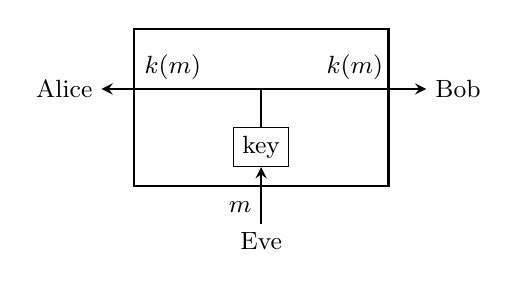
\begin{tikzpicture}[
sArrow/.style={->,>=stealth,thick},
largeResource/.style={draw,thick,minimum width=1.618*2cm,minimum height=2cm}]

\small

\def\u{.236} %2/1.618-1

\node[largeResource] (keyBox) at (0,0) {};
\node (alice) at (-2.5,\u) {Alice};
\node (bob) at (2.5,\u) {Bob};
\node (eve) at (0,-1.7) {Eve};
\node[draw] (key) at (0,-.5) {key};

\draw[sArrow,<->] (alice) to node[pos=.22,auto] {$k(m)$} node[pos=.78,auto] {$k(m)$} (bob);
\draw[thick] (0,\u) to (key);
\draw[sArrow] (eve) to node[pos=.3,auto] {$m$} (key);

\end{tikzpicture}

\caption[Secret key resource with adaptive
length]{\label{fig:qkd.resource.adaptive}A secret key resource with   adaptive key length. This resources allows Eve to choose the length $m$   of the final key $k$, which is then output at Alice's and Bob's interfaces.}
\end{figure}

Such an ideal resource has been considered in \textcite{BHLMO05,HT12}. The reduction from the corresponding security definition in AC to a trace distance criterion still goes through. But instead of \eqnref{eq:d}, we get 
\begin{equation} \label{eq:adpative.trace.d}
\sum_m p_m D \left( \rho^m_{KE},\tau^m_K \otimes \rho^m_E \right) \leq
\eps,
\end{equation}
where $p_m$ is the probability of obtaining a key of length $m$, $\rho^m_{KE}$ is the joint state of the key and Eve's system conditioned on the key having length $m$,  and $\tau^m_K$ is a fully mixed state of dimension $2^m$.


\subsection{Source of entanglement}
\label{sec:alternative.entanglement}

In contrast to \emph{prepare\-/and\-/measure} protocols,
\emph{entanglement\-/based} protocols, e.g., \textcite{Eke91,BBM92},
use a source of entanglement, instead of a quantum communication
channel. It is also pretty standard in security proofs to first
transform a given prepare\-/and\-/measure protocol into an
entanglement\-/based one, and then prove the security of the
latter~\cite{SP00}. In \figref{fig:qkd.real.ent} we draw the system
consisting of a QKD protocol $(\pi^{\qkd}_A,\pi^{\qkd}_B)$, the
authentic channel $\aA$ and a source  $\aE$ of entangled states, which may be
controlled by Eve. To specify the completeness property, we also consider
a source of entanglement $\aE'$ that produces a fixed bipartite
entangled state instead of allowing Eve to decide.

\begin{figure}[tb]


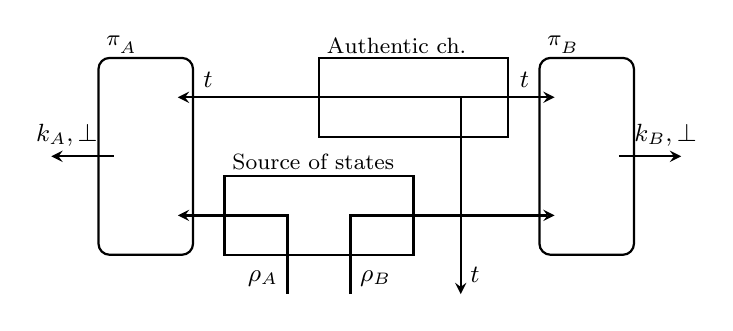
\begin{tikzpicture}[
sArrow/.style={->,>=stealth,thick},
thinResource/.style={draw,thick,minimum width=2.4cm,minimum height=1cm},
protocol/.style={draw,rounded corners,thick,minimum width=1.2cm,minimum height=2.5cm},
pnode/.style={minimum width=.8cm,minimum height=.5cm}]

\small

\def\t{4} %.6+1.2+.4+1.2*3/2
\def\u{2.8} %1.2/2+.4+1.2*3/2
\def\v{.75}
\def\w{.6} %1.2/2

\node[pnode] (a1) at (-\u,\v) {};
\node[pnode] (a2) at (-\u,0) {};
\node[pnode] (a3) at (-\u,-\v) {};
\node[protocol] (a) at (-\u,0) {};
\node[yshift=-2,above right] at (a.north west) {\footnotesize
  $\pi^{\qkd}_A$};
\node (alice) at (-\t,0) {};

\node[pnode] (b1) at (\u,\v) {};
\node[pnode] (b2) at (\u,0) {};
\node[pnode] (b3) at (\u,-\v) {};
\node[protocol] (b) at (\u,0) {};
\node[yshift=-2,above right] at (b.north west) {\footnotesize $\pi^{\qkd}_B$};
\node (bob) at (\t,0) {};

\node[thinResource] (cch) at (\w,\v) {};
\node[yshift=-2,above right] at (cch.north west) {\footnotesize
  Authentic ch.~$\aA$};
\node[thinResource] (qch) at (-\w,-\v) {};
\node[yshift=-1.5,above right] at (qch.north west) {\footnotesize
  Source of states $\aE$};
\node (eveq1) at (-\w-.4,-1.75) {};
\node (junc1) at (eveq1 |- a3) {};
\node (eveq2) at (-\w+.4,-1.75) {};
\node (junc2) at (eveq2 |- a3) {};
\node (evec) at (\w+\w,-1.75) {};
\node (junc3) at (evec |- b1) {};

\draw[sArrow,<->] (a1) to node[auto,pos=.08] {$t$} node[auto,pos=.92] {$t$}  (b1);
\draw[sArrow] (junc3.center) to node[auto,pos=.9] {$t$} (evec.center);

\draw[sArrow] (a2) to node[auto,pos=.75,swap] {$k_{A},\bot$} (alice.center);
\draw[sArrow] (b2) to node[auto,pos=.75] {$k_{B},\bot$} (bob.center);

\draw[sArrow,<-] (a3) to (junc1.center) to node[pos=.8,auto,swap] {$\rho_A$} (eveq1.center);
\draw[sArrow] (eveq2.center) to node[pos=.2,auto,swap] {$\rho_B$} (junc2.center) to (b3);

\end{tikzpicture}


\caption[QKD system with source of
entanglement]{\label{fig:qkd.real.ent}A real QKD system that uses a
  source of entangled states. Instead of having access to an insecure
  channel as in \figref{fig:qkd.real.adv}, Alice and Bob use a source
  of entanglement $\aE$ that is controlled by Eve. This means that Eve may
  generate an arbitrary state $\rho_{ABE}$ of which the $A$ register goes to Alice and
  the $B$ register to Bob.}
\end{figure}

The reduction from the AC security definition to the trace distance criterion described in \secref{sec:security} works here, too, with the source of entanglement replacing the insecure channel, resulting in the same conditions for $\eps$\=/secrecy and $\eps$\=/correctness.

One can also show that any protocol designed for a distributed source
of entanglement can be transformed into one where a state is prepared
locally and sent over an (insecure) channel. To explain this, we first
decompose Alice's QKD protocol in two parts.  In the first she carries
out a subprotocol $\alpha$ that performs a measurement
$\bM^a = \{M^a_x\}_x$ on the state received from the source of
entangled states, where $\bM^a$ is chosen with some probability $p_a$
from a set $\{\bM^a\}_a$. The second part consists of the rest of her
QKD protocol. We illustrate this in \figref{fig:qkd.ent.protocol}.

\begin{figure}[tb]


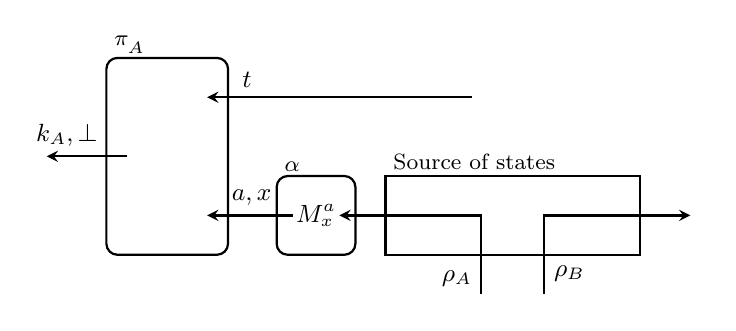
\begin{tikzpicture}[
sArrow/.style={->,>=stealth,thick},
thinResource/.style={draw,thick,minimum width=1.618*2cm,minimum height=1cm},
protocol/.style={draw,rounded corners,thick,minimum width=1.545cm,minimum height=2.5cm},
pnode/.style={minimum width=1cm,minimum height=.5cm},
sqResource/.style={draw,rounded corners,thick,minimum width=1cm,minimum height=1cm}]

\small

\def\t{5.92} %.75+1.545+.5+1+.5+1.618
\def\u{4.39} %1.545/2+.5+1+.5+1.618
\def\um{2.5} %1/2+.5+1.618-.1
\def\ub{2.37} %1.618+.75
\def\v{.75}


\node[pnode] (a1) at (-\u,\v) {};
\node[pnode] (a2) at (-\u,0) {};
\node[pnode] (a3) at (-\u,-\v) {};
\node[protocol] (a) at (-\u,0) {};
\node[yshift=-2,above right] at (a.north west) {\footnotesize
  $\pi^{\qkd}_A$};
\node (alice) at (-\t,0) {};

\node (b1) at (-.4,0 |- a1) {};
\node (b3) at (\ub,-\v) {};

\node[sqResource] (m) at (-\um,-\v) {};
\node[inner sep=1] (mInner) at (-\um,-\v) {$M^a_x$};
\node[yshift=-2,above right] at (m.north west) {\footnotesize
  $\alpha$};

\node[thinResource] (qch) at (0,-\v) {};
\node[yshift=-1.5,above right] at (qch.north west) {\footnotesize
  Source of states $\aE$};
\node (eveq1) at (-.4,-1.75) {};
\node (junc1) at (eveq1 |- a3) {};
\node (eveq2) at (.4,-1.75) {};
\node (junc2) at (eveq2 |- a3) {};

\draw[sArrow] (b1) to node[auto,pos=.85,swap] {$t$}  (a1);

\draw[sArrow] (a2) to node[auto,pos=.75,swap] {$k_{A},\bot$} (alice.center);

\draw[sArrow] (mInner) to node[swap,auto,pos=.48] {$a,x$} (a3);
\draw[sArrow,<-] (mInner) to (junc1.center) to node[pos=.8,auto,swap] {$\rho_A$} (eveq1.center);
\draw[sArrow] (eveq2.center) to node[pos=.264,auto,swap] {$\rho_B$} (junc2.center) to (b3);

\end{tikzpicture}


\caption[Entanglement based QKD
protocol]{\label{fig:qkd.ent.protocol}We split Alice's part of an
  entanglement\-/based QKD protocol in two parts, the measurement of
  the incoming states (denoted by $\alpha$) and the rest of the
  protocol (denoted by $\pi^{\qkd}_A$).}
\end{figure}

We now need to argue that there exists a converter $\gamma$ which constructs
$\alpha \aE$ from an insecure channel $\aQ$ and $\alpha \aE'$ from a
noiseless channel $\aQ'$. For this, we must
establish the two following conditions.
\begin{enumerate}[label=(\roman*), ref=\roman*]
\item \label{eq:ent.sec} There exists a simulator $\sigma_E$ such that
  \[ 
   \gamma \aQ = \alpha \aE \sigma_E.
\]
\item \label{eq:ent.cor} The following equality holds,
  \[\gamma \aQ' = \alpha \aE'.\] 
\end{enumerate}
Once we have established these conditions, it follows immediately from
the composition theorem of the AC framework~\cite{MR11} that any QKD
protocol which is sound when using $\alpha\aE$ and complete when using
$\alpha\aE'$ is also sound and complete when using $\gamma\aQ$ and
$\gamma\aQ'$, respectively.

Let $\rho_{AB}$ be the bipartite entangled state that is generated by
$\aE'$. Let
$\tilde{\varphi}^{x,a}_B \coloneqq \trace[A]{M^a_x \rho_{AB}
  \hconj{\left(M^a_x\right)}}$,
$p_{x|a} \coloneqq \tr \tilde{\varphi}^{x,a}_B$ and
$\varphi^{x,a}_B \coloneqq \tilde{\varphi}^{x,a}_B/p_{x|a}$. We define
the converter $\gamma$ to prepare the state $\varphi^{x,a}_B$ with
probability $p_ap_{x|a}$, which it sends on the insecure
channel. Furthermore, we define the simulator $\sigma_E$ to prepare
$\rho_{AB}$, input the $A$\=/part on the entanglement resource for
Alice and output the $B$\=/part at the outer interface. It is then
straightforward to check from \figref{fig:qkd.ent} that this satisfies
the conditions \eqref{eq:ent.sec} and \eqref{eq:ent.cor} described above.


\begin{figure*}[htb]
\centering
\subfloat[Soundness][\label{fig:qkd.ent.soundness}When modeling
  soundness, the adversary can modify the messages on the insecure
  channel $\aQ$. The simulator $\sigma_E$ generates the entangled state
  $\rho_{AB}$ that is expected from of a non\-/adversarial source of
  entangled states, and outputs the $B$ part at the outer interface,
  making the two systems on the left and right indistinguishable.]{
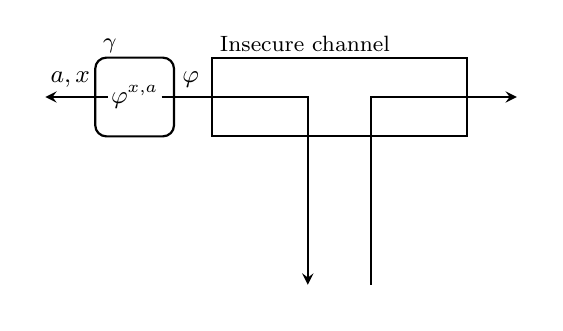
\begin{tikzpicture}[
sArrow/.style={->,>=stealth,thick},
thinResource/.style={draw,thick,minimum width=1.618*2cm,minimum height=1cm},
sqResource/.style={draw,rounded corners,thick,minimum width=1cm,minimum height=1cm}]

\small

\def\ua{3.85} %.75+1+.5+1.618
\def\um{2.6} %1/2+.5+1.618
\def\ub{2.37} %1.618+.75
\def\t{2.5}

\node (a) at (-\ua,0) {};
\node (b) at (\ub,0) {};

\node[sqResource] (m) at (-\um,0) {};
\node[inner sep=1] (mInner) at (-\um,0) {$\varphi^{x,a}$};
\node[yshift=-2,above right] at (m.north west) {\footnotesize
  $\gamma$};

\node[thinResource] (qch) at (0,0) {};
\node[yshift=-1.5,above right] at (qch.north west) {\footnotesize
  Insecure channel $\aQ$};

\node (le) at (-.4,-\t) {};
\node (re) at (.4,-\t) {};

\node (junc1) at (le |- a) {};
\node (junc2) at (re |- a) {};

\draw[sArrow] (mInner) to node[swap,auto,pos=.6] {$a,x$} (a);

\draw[sArrow] (mInner) to node[auto,pos=.2] {$\varphi$} (junc1.center) to (le);
\draw[sArrow] (re) to (junc2.center) to (b);

\end{tikzpicture}  \hspace{2cm}
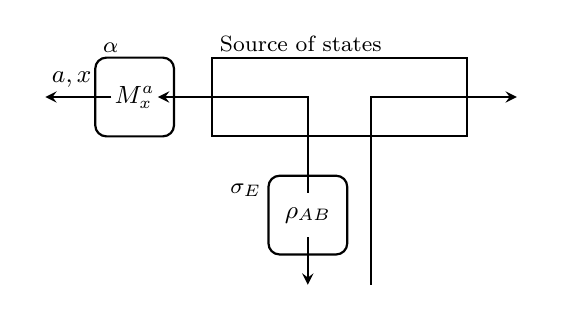
\begin{tikzpicture}[
sArrow/.style={->,>=stealth,thick},
thinResource/.style={draw,thick,minimum width=1.618*2cm,minimum height=1cm},
sqResource/.style={draw,rounded corners,thick,minimum width=1cm,minimum height=1cm}]

\small

\def\ua{3.85} %.75+1+.5+1.618
\def\um{2.6} %1/2+.5+1.618
\def\ub{2.37} %1.618+.75
\def\v{.75}
\def\t{2.5}

\node (a) at (-\ua,0) {};
\node (b) at (\ub,0) {};

\node[sqResource] (m) at (-\um,0) {};
\node[inner sep=1] (mInner) at (-\um,0) {$M^a_x$};
\node[yshift=-2,above right] at (m.north west) {\footnotesize
  $\alpha$};

\node[thinResource] (qch) at (0,0) {};
\node[yshift=-1.5,above right] at (qch.north west) {\footnotesize
  Source of states $\aE$};

\node[sqResource] (sim) at (-.4,-2*\v) {};
\node[inner sep=5] (simInner) at (-.4,-2*\v) {$\rho_{AB}$};
\node[xshift=1,below left] at (sim.north west) {\footnotesize $\sigma_E$};

\node (le) at (-.4,-\t) {};
\node (re) at (.4,-\t) {};

\node (junc1) at (le |- a) {};
\node (junc2) at (re |- a) {};

\draw[sArrow] (mInner) to node[swap,auto,pos=.6] {$a,x$} (a);

\draw[sArrow,<-] (mInner) to (junc1.center) to (simInner);
\draw[sArrow] (simInner) to (le);
\draw[sArrow] (re) to (junc2.center) to (b);

\end{tikzpicture}}

\vspace{12pt}

\subfloat[Completeness][\label{fig:qkd.ent.completeness}When modeling
completeness, the source of entanglement $\aE'$ prepares the state
$\rho_{AB}$. The systems on the left and right are
indistinguishable.]{
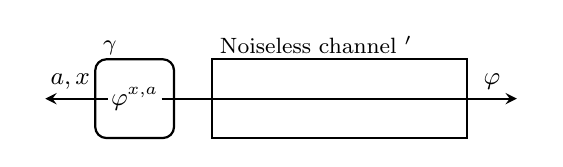
\begin{tikzpicture}[
sArrow/.style={->,>=stealth,thick},
thinResource/.style={draw,thick,minimum width=1.618*2cm,minimum height=1cm},
% filter/.style={draw,thick,minimum width=1.618cm,minimum height=1cm},
sqResource/.style={draw,rounded corners,thick,minimum width=1cm,minimum height=1cm}]

\small

\def\ua{3.85} %.75+1+.5+1.618
\def\um{2.6} %1/2+.5+1.618
\def\ub{2.37} %1.618+.75
\def\v{.75}

\node (a) at (-\ua,0) {};
\node (b) at (\ub,0) {};

\node[sqResource] (m) at (-\um,0) {};
\node[inner sep=1] (mInner) at (-\um,0) {$\varphi^{x,a}$};
\node[yshift=-2,above right] at (m.north west) {\footnotesize
  $\gamma$};

\node[thinResource] (qch) at (0,0) {};
\node[yshift=-1.5,above right] at (qch.north west) {\footnotesize
  Noiseless channel $\aQ'$};

% \node[filter] (qchf) at (0,-2*\v) {};
% \node[xshift=2,below left] at (qchf.north west) {\footnotesize $\sharp_E$};

% \node[xshift=-.4cm] (qchfl) at (qchf.center) {};
% \node[xshift=.4cm] (qchfr) at (qchf.center) {};
% \node (qchl) at (qchfl |- qchf.north) {};
% \node (qchr) at (qchfr |- qchf.north) {};
% \node (junc1) at (qchfl |- a) {};
% \node (junc2) at (qchfr |- a) {};

\draw[sArrow] (mInner) to node[swap,auto,pos=.6] {$a,x$} (a);

\draw[sArrow] (mInner) to node[auto,pos=.93] {$\varphi$} (b);

% \draw[sArrow] (qchl.center) to (qchfl.center) to (qchfr.center) to (qchr.center);

\end{tikzpicture} \hspace{2cm}
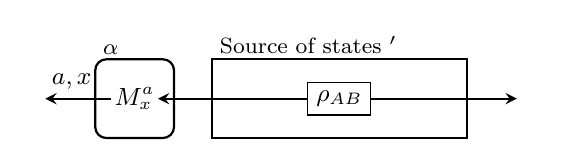
\begin{tikzpicture}[
sArrow/.style={->,>=stealth,thick},
thinResource/.style={draw,thick,minimum width=1.618*2cm,minimum height=1cm},
% filter/.style={draw,thick,minimum width=1.618cm,minimum height=1cm},
sqResource/.style={draw,rounded corners,thick,minimum width=1cm,minimum height=1cm}]

\small

\def\ua{3.85} %.75+1+.5+1.618
\def\um{2.6} %1/2+.5+1.618
\def\ub{2.37} %1.618+.75
\def\v{.75}

\node (a) at (-\ua,0) {};
\node (b) at (\ub,0) {};

\node[sqResource] (m) at (-\um,0) {};
\node[inner sep=1] (mInner) at (-\um,0) {$M^a_x$};
\node[yshift=-2,above right] at (m.north west) {\footnotesize
  $\alpha$};

\node[thinResource] (qch) at (0,0) {};
\node[yshift=-1.5,above right] at (qch.north west) {\footnotesize
  Source of states $\aE'$};

% \node[filter] (qchf) at (0,-2*\v) {};
% \node[xshift=2,below left] at (qchf.north west) {\footnotesize $\lozenge_E$};
\node[draw] (boxState) at (0,0) {$\rho_{AB}$};

% \node[xshift=-.4cm] (qchfl) at (qchf.center) {};
% \node[xshift=.4cm] (qchfr) at (qchf.center) {};
% \node (qchl) at (qchfl |- qchf.north) {};
% \node (qchr) at (qchfr |- qchf.north) {};
% \node (junc1) at (qchfl |- a) {};
% \node (junc2) at (qchfr |- a) {};

\draw[sArrow] (mInner) to node[swap,auto,pos=.6] {$a,x$} (a);

\draw[sArrow] (boxState) to (mInner);
\draw[sArrow] (boxState) to (b);

% \draw[sArrow,<->] (qchl.center) to (qchfl.center) to (qchfr.center) to (qchr.center);

\end{tikzpicture}}

\caption[Using an entanglement protocol with an insecure
channel]{\label{fig:qkd.ent}Pictorial proof for the security of the
  construction of $\alpha\aE$ from $\aQ$ and $\alpha \aE'$ from
  $\aQ'$. Any protocol designed to run with a source of entangled
  states $\aE$ and which measures the incoming states on Alice's side
  as does $\alpha$ can be equivalently used with an insecure channel
  $\aQ$ and a converter $\gamma$ that generates the states to be sent
  on the channel.}
\end{figure*}

\subsection{Imperfect randomness}
\label{sec:alternative.randomness}

QKD protocols usually assume that the honest parties have (arbitrary) access to perfect random numbers. This is however never the case in practice. A more realistic model of a QKD system would consider randomness as a resource that is available in limited and imperfect quantities to Alice and Bob. The real QKD setting drawn in \figref{fig:qkd.real} needs to be changed to take this into account. In \figref{fig:qkd.real.randomness} we depict a QKD protocol that \--- additionally to the insecure quantum channel and authentic classical channel \--- has access to resources producing (local) randomness, $\aR_A$ and $\aR_B$, at Alice's and Bob's interfaces, respectively. A different model of randomness resources might also provide some partial (quantum) information about the randomness to the eavesdropper. For simplicity, however, we chose to draw the simpler case in which $\aR_A$ and $\aR_B$ have an empty interface for the dishonest party.

\begin{figure}[tb]


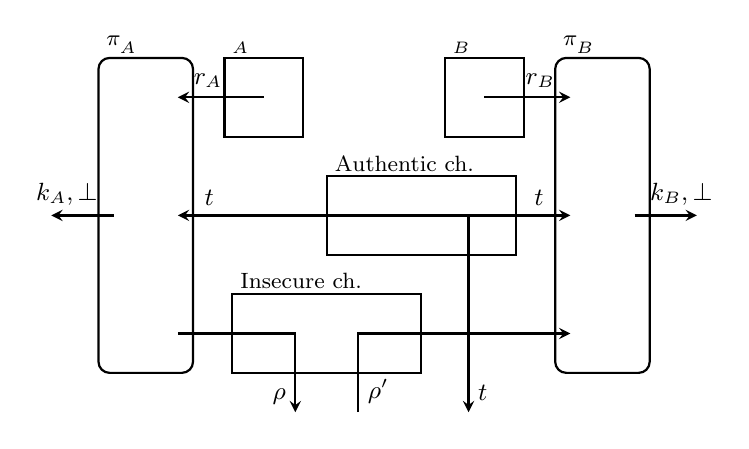
\begin{tikzpicture}[
sArrow/.style={->,>=stealth,thick},
thinResource/.style={draw,thick,minimum width=2.4cm,minimum height=1cm},
pnode/.style={minimum width=.8cm,minimum height=.5cm},
sqResource/.style={draw,thick,minimum width=1cm,minimum height=1cm},
longProtocol/.style={draw,rounded corners,thick,minimum width=1.2cm,minimum height=4cm}]


\small

\def\t{4.1} %.6+1.2+.5+1.2*3/2
\def\u{2.9} %1.2/2+.5+1.2*3/2
\def\v{1.5}
\def\w{.6} %1.2/2
\def\x{.8} %1.2-.4


\node[pnode] (a1) at (-\u,\v) {};
\node[pnode] (a2) at (-\u,0) {};
\node[pnode] (a3) at (-\u,-\v) {};
\node[longProtocol] (a) at (-\u,0) {};
\node[yshift=-2,above right] at (a.north west) {\footnotesize
  $\pi^{\qkd}_A$};
\node (alice) at (-\t,0) {};

\node[pnode] (b1) at (\u,\v) {};
\node[pnode] (b2) at (\u,0) {};
\node[pnode] (b3) at (\u,-\v) {};
\node[longProtocol] (b) at (\u,0) {};
\node[yshift=-2,above right] at (b.north west) {\footnotesize $\pi^{\qkd}_B$};
\node (bob) at (\t,0) {};

\node[sqResource] (ra) at (-\x-\w,\v) {};
\node[yshift=-2,above right] at (ra.north west) {\footnotesize $\aR_A$};
\node[sqResource] (rb) at (\x+\w,\v) {};
\node[yshift=-2,above right] at (rb.north west) {\footnotesize $\aR_B$};
\node[thinResource] (cch) at (\w,0) {};
\node[yshift=-2,above right] at (cch.north west) {\footnotesize
  Authentic ch.~$\aA$};
\node[thinResource] (qch) at (-\w,-\v) {};
\node[yshift=-1.5,above right] at (qch.north west) {\footnotesize
  Insecure ch.~$\aQ$};
\node (eveq1) at (-\w-.4,-\v-1) {};
\node (junc1) at (eveq1 |- a3) {};
\node (eveq2) at (-\w+.4,-\v-1) {};
\node (junc2) at (eveq2 |- a3) {};
\node (evec) at (\w+\w,-\v-1) {};
\node (junc3) at (evec |- b2) {};

\draw[sArrow] (ra.center) to node[auto,swap,pos=.65] {$r_A$} (a1);
\draw[sArrow] (rb.center) to node[auto,pos=.65] {$r_B$}  (b1);

\draw[sArrow,<->] (a2) to node[auto,pos=.08] {$t$} node[auto,pos=.92] {$t$}  (b2);
\draw[sArrow] (junc3.center) to node[auto,pos=.9] {$t$} (evec.center);

\draw[sArrow] (a2) to node[auto,pos=.75,swap] {$k_{A},\bot$} (alice.center);
\draw[sArrow] (b2) to node[auto,pos=.75] {$k_{B},\bot$} (bob.center);

\draw[sArrow] (a3) to (junc1.center) to node[pos=.8,auto,swap] {$\rho$} (eveq1.center);
\draw[sArrow] (eveq2.center) to node[pos=.264,auto,swap] {$\rho'$} (junc2.center) to (b3);

\end{tikzpicture}



\caption[QKD system with explicit randomness
resource]{\label{fig:qkd.real.randomness} A real QKD system with a
  deterministic protocol $(\pi^{\qkd}_A,\pi^{\qkd}_B)$ and explicit
  sources of randomness $\aR_A$ and $\aR_B$.}
\end{figure}

In such a setting, the converters $\pi^{\qkd}_A$ and $\pi^{\qkd}_B$
are deterministic systems. A QKD protocol would then construct an
ideal key resource given access to these three resources. It remains
an open problem to minimize the assumptions on the sources of
randomness in QKD. Recent results on device\-/independent randomness
amplification~\cite{CR12} show that under certain minimal assumptions\footnote{One
  generally has to assume that no messages leave or enter the quantum
  devices unless authorized by the protocol. Some papers make
  additional assumptions to simplify the protocols and proofs.} about
the workings of an unknown quantum system, one can transform a single
(public) weak source of randomness into a fully (private) random
source~\cite{CSW14,BRGHHHSW16,KAF20}. Alternatively, if two (or more)
sources of weak randomness are available to a player (under certain
strict conditions on the correlations between these different
sources), these can be combined to obtain (approximately) uniform
randomness \cite{CLW14,AFPS16}. Composing this with a standard QKD
protocol would allow secret keys to be distributed when only weak
randomness is available to the honest parties.


\subsection{Device-independent QKD}
\label{sec:alternative.di}

In this review we have so far always considered scenarios for which it
is assumed that the players have trusted quantum devices, which work
exactly according to their specifications. For instance, if a player
instructs the device to generate a $\zero$ state, then it is assumed
that the device generates precisely this state. This assumption is
however not met in any actual implementation with realistic devices,
as these are never perfect. Indeed, there have been numerous
demonstrations of successful attacks against implementations of
quantum cryptographic protocols that exploited deviations of the
devices' functionality from the specifications, as discussed in
\secref{sec:attacks}. Crucially, this problem cannot be solved only by
a more careful design of the devices, for it appears to be impossible
to guarantee their perfect working under all possible environmental
conditions.

A theoretical solution to this problem is to devise protocols whose
security does not rely on the assumption that devices are perfect.
Ideally, they should provide security guarantees even if the devices
are untrusted, meaning that their behavior may deviate arbitrarily
from the specification. Remarkably, using quantum devices, this is
possible (with certain caveats described below). The idea is to use a
phenomenon called \emph{(Bell) non\-/locality} \cite{Bell64} \--- see
also \textcite{Sca13,BCPSW14} for review articles on the topic. The
subfield of cryptography that studies the use of non\-/locality to
design protocols that work with untrusted devices is termed
\emph{device\-/independent cryptography}.
  
In a nutshell, a Bell inequality is a bound on the probability of
observing certain values in an experiment involving measurements of two isolated (and hence non-communicating) systems. The bound characterises classical locality: it cannot be violated if
the two isolated systems are described by classical physics. However, the bound can be violated by measurements on entangled quantum systems.   One of the most commonly used Bell inequalities is the
CHSH inequality \cite{CHSH69}. It states that, if two players each
hold non\-/communicating systems, and each performs one out of two
binary measurements chosen uniformly at random on their respective
system, where the choice of the measurement is given by
$x,y \in \{0,1\}$ and the outcome is given by $a,b \in \{0,1\}$,
respectively, then the probability that $xy = a \xor b$ should be less than
or equal to $3/4$.\footnote{An alternative formulation of the
  inequality is
  $\left| E(0,0) + E(0,1) + E(1,0) - E(1,1) \right| \leq 2$, where
  $E(x,y)$ is the expected value of the product of the outcomes of the
  systems when measured with settings $x$ and $y$, respectively, and
  the outcomes are values in $\{-1,+1\}$.} But if the systems are
quantum, it is possible to observe this outcome with probability up to
$\approx .85$ \--- this is achieved if the systems are in a perfectly
entangled state and the players perform an optimal measurement.

An observation of a violation of a Bell inequality implies that the
measurement outcomes contain some genuine randomness
\cite{Col06,PAM10,AMP12,CR12}, even conditioned on the knowledge of
the person who set up and programmed the devices used in the
experiment \--- the only assumptions being that no information other
than the measurement result leaves the devices, and that these devices
never fall in the hands of an adversary, since their internal memory
may contain a copy of the measurement outcomes. This randomness may
then be used to generate uniform random numbers
\cite{VV12,CSW14,MS14,BRGHHHSW16,KAF20} or a shared secret key
\cite{BHK05,PABGMS09,VV14,ADFRV18,AFRV19}.

For a review of different results and techniques in
device\-/independent cryptography, we refer to \textcite{ER14}. In
this section we show how to model device\-/independent quantum key
distribution (DI-QKD) in the AC framework. It then follows from the
composition theorem of AC, that the resulting key can be safely used
in applications requiring one.

The converters $\pi^\qkd_A$ and $\pi^\qkd_B$ modeling Alice's and
Bob's parts of the protocol in \secref{sec:qkd} are systems which
generate quantum states and perform measurements. In DI-QKD, exactly
these operations cannot be trusted. So instead, the DI protocol
$(\pi^\diqkd_A,\pi^\diqkd_B)$ will only involve \emph{classical}
operations. Everything \emph{quantum} is moved into a resource, a
device $\aD$. The honest players can send bits to these devices, and
receive bits back from them \--- this corresponds to choosing a
measurement $x,y \in \{0,1\}$ and receiving the outcome
$a,b \in \{0,1\}$, described a few paragraphs earlier. The adversary is
permitted to ``program'' these devices by providing some initial state
$\rho$ as input \--- depending on the model, Eve may be allowed to
provide further inputs to the device at some later point, e.g., to
provide more EPR pairs so that it may continue running. The
corresponding real world is drawn in
\figref{fig:alternatives.diqkd}. The ideal world will be identical to
that of standard QKD, since we wish to construct the same key
resource, i.e., \figref{fig:qkd.resource.sim}.


\begin{figure}[tb]

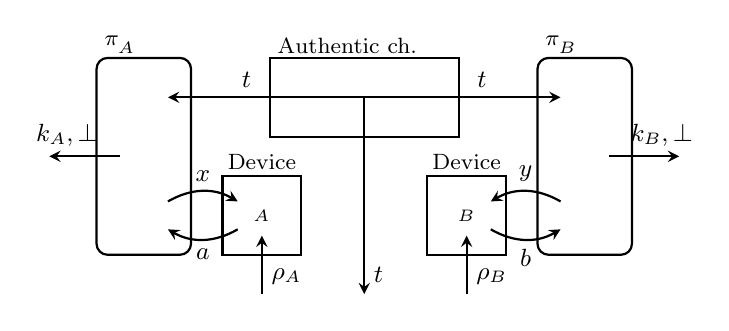
\begin{tikzpicture}[
sArrow/.style={->,>=stealth,thick},
thinResource/.style={draw,thick,minimum width=2.4cm,minimum height=1cm},
sqResource/.style={draw,thick,minimum width=1cm,minimum height=1cm},
protocol/.style={draw,rounded corners,thick,minimum width=1.2cm,minimum height=2.5cm},
pnode/.style={minimum width=.6cm,minimum height=.5cm}]

\small

\def\t{4} %.6+1.2+.4+1.2*3/2
\def\u{2.8} %1.2/2+.4+1.2*3/2
\def\v{.75}
\def\w{1.3} 

\node[pnode] (a1) at (-\u,\v) {};
\node[pnode] (a2) at (-\u,0) {};
\node[pnode] (a3) at (-\u,-\v) {};
\node[protocol] (a) at (-\u,0) {};
\node[yshift=-2,above right] at (a.north west) {\footnotesize
  $\pi^{\diqkd}_A$};
\node (alice) at (-\t,0) {};

\node[pnode] (b1) at (\u,\v) {};
\node[pnode] (b2) at (\u,0) {};
\node[pnode] (b3) at (\u,-\v) {};
\node[protocol] (b) at (\u,0) {};
\node[yshift=-2,above right] at (b.north west) {\footnotesize $\pi^{\diqkd}_B$};
\node (bob) at (\t,0) {};

\node[thinResource] (cch) at (0,\v) {};
\node[yshift=-2,above right] at (cch.north west) {\footnotesize
  Authentic ch.~$\aA$};
\node[sqResource] (da) at (-\w,-\v) {$\aD_A$};
\node[yshift=-1.5,above] at (da.north) {\footnotesize
  Device};
\node[pnode] (dan) at (-\w,-\v) {};
\node[sqResource] (db) at (\w,-\v) {$\aD_B$};
\node[yshift=-1.5,above] at (db.north) {\footnotesize
  Device};
\node[pnode] (dbn) at (\w,-\v) {};

\node (eveq1) at (-\w,-1.75) {};
\node (eveq2) at (\w,-1.75) {};
\node (evec) at (0,-1.75) {};
\node (junc3) at (evec |- b1) {};

\draw[sArrow,<->] (a1) to node[auto,pos=.2] {$t$} node[auto,pos=.8] {$t$}  (b1);
\draw[sArrow] (junc3.center) to node[auto,pos=.9] {$t$} (evec.center);

\draw[sArrow] (a2) to node[auto,pos=.75,swap] {$k_{A},\bot$} (alice.center);
\draw[sArrow] (b2) to node[auto,pos=.75] {$k_{B},\bot$} (bob.center);

\draw[sArrow] (eveq1.center) to node[pos=.3,auto,swap] {$\rho_A$} (dan);
\draw[sArrow] (eveq2.center) to node[pos=.3,auto,swap] {$\rho_B$} (dbn);

\draw[sArrow,bend left] (a3) to node[pos=.5,auto] {$x$} (dan);
\draw[sArrow,bend left] (dan) to node[pos=.5,auto] {$a$} (a3);
\draw[sArrow,bend right] (b3) to node[pos=.5,auto,swap] {$y$} (dbn);
\draw[sArrow,bend right] (dbn) to node[pos=.5,auto,swap] {$b$} (b3);

\end{tikzpicture}


\caption[DI-QKD]{\label{fig:alternatives.diqkd}The real world setting
  for  a DI-QKD protocol. Eve can program the devices $\aD$, but cannot
  receive any output from them.}
\end{figure}

Applying \defref{def:security}, this means that the protocol
$(\pi^\diqkd_A,\pi^\diqkd_B)$ constructs $\aK$ from $\aA$, $\aD_A$ and
$\aD_B$ within $\eps$ if
\begin{equation} \label{eq:diqkd}
  \exists \sigma_E, \quad \pi_A^{\diqkd}\pi_B^{\diqkd}(\aD_A \| \aD_B \| \aA)
  \close{\eps} \aK \sigma_E.
\end{equation}
Note that we have not specified the behaviors of the devices $\aD_A$
and $\aD_B$ at all. In fact, we need \eqnref{eq:diqkd} to hold for all
devices $\aD_A$ and $\aD_B$.\footnote{The simulator may depend on
  these devices, i.e., $\forall \aD_A, \aD_B, \exists \sigma_E$ such
  that \eqnref{eq:diqkd} holds.} This is exactly the
\emph{device\-/independant} guarantee, namely that security holds
regardless of how the (quantum) devices work. Alternatively one can
consider fixed devices $\aD_A$ and $\aD_B$ that are universal
computers, and have their program be part of the inputs at the $E$ interface.

As usual, completeness is captured by specific devices $\aD'_A$ and
$\aD'_B$ that work honestly \--- e.g., they share perfectly entangled
states and perform the correct measurements as specified by the
protocol \--- as well as the same honest resources $\aA'$ and $\aK'$
as in \secref{sec:qkd}. Additionally to
\eqnref{eq:diqkd}, we also need
\begin{equation*} %\label{eq:qkd.robust}
  \pi_A^{\diqkd}\pi_B^{\diqkd}(\aD'_A \| \aD'_B
  \| \aA') \close{\eps'} \aK'.
\end{equation*}

The same reduction as for (normal) QKD goes through, and one can show
that \eqnref{eq:diqkd} is satisfied if for all behaviors of the
devices (and their inputs), \eqnsref{eq:qkd.cor} and \eqref{eq:qkd.sec}
hold.

Note however that the construction outlined in this section only
allows the devices $\aD_A$ and $\aD_B$ to be accessed during the
protocol. No access is granted after the protocol ends, meaning that
we make no security statement about what happens if the devices are
reused. It is an open question how to reuse devices in DI
cryptography, which we discuss in \secref{sec:open.di}.

Proving security of device-independent QKD is more challenging than in
the device-dependent case. One of the difficulties is that the
measurement operators that describe Alice and Bob's measurement can be
arbitrary. In particular it cannot be assumed, for instance, that two
subsequent measurement outcomes by Bob are obtained by two separate
measurement processes. While some of the techniques described
in~\secref{sec:securityproofs}, such as entropy accumulation, are
still applicable to the device-independent setting, others, like de
Finetti-type theorems, are not or must be adapted,
[see~\textcite{ArnonThesis} for details].

\subsection{Semi-device-independent QKD}
\label{sec:alternative.semi}

The only assumption made about the devices in DI-QKD is that no
information leaves these devices unless allowed by the protocols (see
\secref{sec:alternative.di}). But achieving the violation of Bell
inequalities needed for this is challenging because it requires high
detector efficiency and tolerates only low noise on the
channel~\cite{BCPSW14}. Protocols that are easier to implement can be
achieved by making additional assumptions about the quantum devices
used by Alice and Bob. These are generally called
\emph{semi\-/device\-/independent} (semi-DI).

Many different assumptions may be labeled semi-DI. For example, in a
one-sided device-independent setting the protocol is DI for Bob but
not for Alice \cite{BCWSW12}. One may also assume dimension bounds on
the quantum systems generated by untrusted devices as in
\textcite{PB11}. Alternatively, \textcite{LPTRG13} assume that each
use of the devices are causally independent \--- i.e., the states
generated and measurements performed are in product form \--- to
analyze a protocol where the Bell violation is measured locally in
Alice's lab, thus avoiding the noise introduced by the channel between
Alice and Bob. Similar ideas have been used for other protocols than
QKD, e.g., semi-DI quantum money~\cite{HS20,BDG19}.

One of the most promising forms of semi-DI QKD, which has already been
implemented over large distances
\cite{Liu13,Tang2014,Pirandola2015,Yin2016} is
\emph{measurement\-/device\-/independent} (MDI) QKD
\cite{LCQ12,BP12,MR12,CXCLTL14}. Here, one assumes that players can
generate the states they desire, but one does not trust measurement
devices at all. This model is motivated by the attacks on the
detectors, e.g., the time-shift attacks or detector blinding attacks
discussed in \secref{sec:attacks:hacking}.

To understand how such protocols work, we will start from an
entanglement based protocol as in
\secref{sec:alternative.entanglement}, then modify it step by
step, until we achieve a prepare\-/and\-/measure protocol, in which
all measurements are performed by the adversary. Since the final
protocol is as secure as the original one, and the original one is
secure for all adversaries, the final MDI QKD protocol is secure
for all adversaries as well. In particular, it is secure for
adversaries that completely control the measurement apparatus.

In an entanglement based protocol, Alice and Bob receive the $A$ and
$B$ parts of a state $\psi_{ABR}$, and measure these systems in either
the computational or diagonal basis, obtaining a raw key. This key is
then processed as in a prepare\-/and\-/measure protocol (see
\secref{sec:qkd.protocol} and \secref{sec:securityproofs}).  If the
source gave them a state which is (close to) a tensor product of EPR
pairs, such a protocol is guaranteed to terminate with a shared secret
key. Equivalently, the source could generate any of the Bell states,
and notify Alice and Bob which one it gave them. They then perform bit
or phase flips to change it to an EPR pair.

Instead of the source distributing an entangled state, Alice and Bob
could each generate an EPR pair $AA'$ and $BB'$, respectively. They
then send $A'$ and $B'$ to a third party, Charlie, who measures this
in the Bell basis, and tells them the measurement outcome. If
performed correctly, the $AB$ system will be in a Bell state, and the
measurement outcome will tell them which one. By flipping bits or
phases, Alice and Bob can turn this into an EPR pair, and continue
with the protocol as above. Crucially, if Charlie does not perform the
correct measurement, then Alice and Bob will end up holding the $A$
and $B$ parts of some unknown state $\psi_{ABR}$. But this does not
compromise security: if it is too far from the expected state, the
protocol will just abort.

Instead of first performing a bit or phase flip, and then measuring,
Alice and Bob could first measure their systems $A$ and $B$, and then
flip the value of the measurement outcome if needed. And instead of
generating EPR pairs $AA'$ and $BB'$, then measuring $A$ and $B$, they
could pick the measurement outcome at random, then generate the
corresponding reduced state in $A'$ and $B'$ respectively, send these
to Charlie, and when they obtain the measurement outcome from Charlie,
they flip their bits if needed.

The only (trusted) quantum operations that Alice and Bob need to
perform in the protocol described in the paragraph above are
generating the states in the systems $A'$ and $B'$. All measurements
have now been delegated to Charlie, who may deviate arbitrarily from
the protocol without compromising security.

The real world for such a MDI-QKD protocol is drawn in
\figref{fig:alternatives.mdi}, where one can see that the converters
$\pi^{\mdi}_A$ and $\pi^{\mdi}_B$ do not have any incoming quantum
states, i.e., they do not need to perform any measurement.

Security proofs for MDI-QKD protocols can be based on the same techniques as those for fully device-independent protocols, as discussed in \secref{sec:alternative.di}. The comments on security proofs made in that section thus also apply here. 

\begin{figure}[tb]

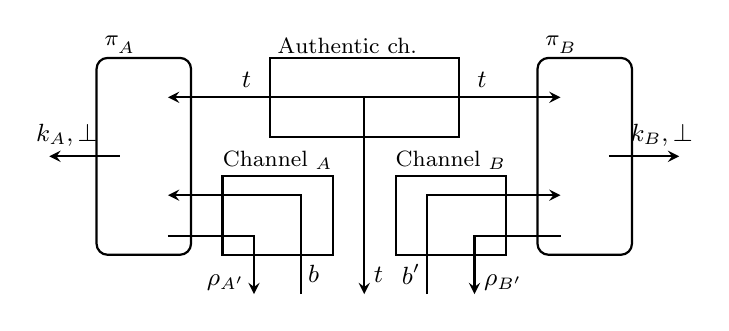
\begin{tikzpicture}[
sArrow/.style={->,>=stealth,thick},
thinResource/.style={draw,thick,minimum width=2.4cm,minimum height=1cm},
sqResource/.style={draw,thick,minimum width=1.4cm,minimum height=1cm},
protocol/.style={draw,rounded corners,thick,minimum width=1.2cm,minimum height=2.5cm},
pnode/.style={minimum width=.6cm,minimum height=.5cm}]

\small

\def\t{4} %.6+1.2+.4+1.2*3/2
\def\u{2.8} %1.2/2+.4+1.2*3/2
\def\v{.75}
\def\w{1.1} 
\def\a{.3}

\node[pnode] (a1) at (-\u,\v) {};
\node[pnode] (a2) at (-\u,0) {};
\node[pnode] (a3) at (-\u,-\v) {};
\node[protocol] (a) at (-\u,0) {};
\node[yshift=-2,above right] at (a.north west) {\footnotesize
  $\pi^{\mdi}_A$};
\node (alice) at (-\t,0) {};

\node[pnode] (b1) at (\u,\v) {};
\node[pnode] (b2) at (\u,0) {};
\node[pnode] (b3) at (\u,-\v) {};
\node[protocol] (b) at (\u,0) {};
\node[yshift=-2,above right] at (b.north west) {\footnotesize $\pi^{\mdi}_B$};
\node (bob) at (\t,0) {};

\node[thinResource] (cch) at (0,\v) {};
\node[yshift=-2,above right] at (cch.north west) {\footnotesize
  Authentic ch.~$\aA$};
\node[sqResource] (da) at (-\w,-\v) {};
\node[yshift=-1.5,above] at (da.north) {\footnotesize
  Channel $\aC_A$};
\node[pnode] (dan) at (-\w,-\v) {};
\node[sqResource] (db) at (\w,-\v) {};
\node[yshift=-1.5,above] at (db.north) {\footnotesize
  Channel $\aC_B$};
\node[pnode] (dbn) at (\w,-\v) {};

\node (eveq11) at (-\w-\a,-1.75) {};
\node (eveq12) at (-\w+\a,-1.75) {};
\node (eveq21) at (\w-\a,-1.75) {};
\node (eveq22) at (\w+\a,-1.75) {};
\node (evec) at (0,-1.75) {};
\node (junc3) at (evec |- b1) {};

\draw[sArrow,<->] (a1) to node[auto,pos=.2] {$t$} node[auto,pos=.8] {$t$}  (b1);
\draw[sArrow] (junc3.center) to node[auto,pos=.9] {$t$} (evec.center);

\draw[sArrow] (a2) to node[auto,pos=.75,swap] {$k_{A},\bot$} (alice.center);
\draw[sArrow] (b2) to node[auto,pos=.75] {$k_{B},\bot$} (bob.center);

\draw[sArrow] (a3.south east) to (eveq11 |- a3.south east) to node[pos=.8,auto,swap] {$\rho_{A'}$} (eveq11.center);
\draw[sArrow] (b3.south west) to (eveq22 |- b3.south west) to node[pos=.8,auto] {$\rho_{B'}$} (eveq22.center);
\draw[sArrow] (eveq12.center) to node[pos=.2,auto,swap,xshift=-1] {$b$} (eveq12 |- a3.north east) to (a3.north east);
\draw[sArrow] (eveq21.center) to node[pos=.2,auto,xshift=1] {$b'$} (eveq21 |- b3.north west) to (b3.north west);

\end{tikzpicture}


\caption[MDI-QKD]{\label{fig:alternatives.mdi}The real world setting
  for a MDI-QKD protocol. The only quantum operations performed by
  $\pi^{\mdi}_A$ and $\pi^{\mdi}_B$ are the generation of quantum
  states. The communication resources $\aC$ send quantum systems from
  Alice or Bob to Eve, and classical bits from Eve to Alice and Bob..}
\end{figure}

\subsection{Memoryless adversaries}
\label{sec:alternative.memoryless}

The previous sections analyzed different models of QKD, in which we
changed the capabilities and resources of the honest players running
the protocol. Similar techniques may also be used to model
limitations on adversaries. In this last section we consider as example QKD
protocol with an adversary that has no (long-term) quantum memory, and is
forced to measure the quantum states exchanged between Alice and Bob
during the QKD protocol and store the classical information.

The insecure channel resource, $\aQ$, modeled as part of the real QKD
system in \figref{fig:qkd.real.adv} gives complete control over the
states sent on this channel to the adversary. Since this may include
storing them and measuring them at a later point, we need to limit the
adversary's access to this channel as part of the insecure channel
resource. We may thus define a different channel $\tilde{\aQ}$, which
requires Eve to input some measurement specification and then obtains
the measurement outcome at her interface. The resulting
post\-/measurement state is then output at Bob's interface.

The model of $\tilde{\aQ}$ described above is just one possible way
one may imagine limiting Eve's access to the states sent during
QKD. The result is a change in the requirements of the QKD
protocol. Instead of constructing a secure key $\aK$ from an authentic
channel $\aA$ and an insecure channel $\aQ$, it is now sufficient if
$\aK$ can be constructed from $\aA$ and $\tilde{\aQ}$. It is not hard
to see that, since the accessible information (see
\secref{sec:qkd.other.ai}) measures the information an adversary has
\emph{after} measuring their quantum states, a QKD protocol with low
accessible information would satisfy such a construction \--- namely,
$\aA \| \tilde{\aQ} \rightarrow \aK$. The accessible information
security measure is thus a composable criterion under the assumption
that the adversary has such a physical limit on their memory.

Since QKD protocols are secure against general adversaries as modeled
in \secref{sec:qkd}, there does not seem to be much incentive to
consider adversaries with limitations on their memory (unlike for some
two-party protocols discussed in \secref{sec:open.other}). It is
however noteworthy that, as already mentioned in
\secref{sec:qkd.other.ac}, by explicitly limiting the adversary's
capabilities we capture weaker security notions that appeared in the literature.


%%% Local Variables:
%%% TeX-master: "main.tex"
%%% End:


%\vspace{-0.05in}
\section{Optimization Algorithm}
\label{sec:algorithm}
\begin{algorithm}[!ht]
\begin{algorithmic}[1]
\Require Query workload $Q$, event stream $I$, \app\ graph $G$, hash table of snapshots $S$
\Ensure Hash table of results $R$ 
\State $G \leftarrow \emptyset$, $S, R \leftarrow$ empty hash tables
\ForAll {event $e \in I$ with $e.type=E$} 
    \State $//$ \textbf{\app\ graph construction}
    \ForAll {$q \in Q$ \text{ with event types }T}
        \ForAll {$E' \in T,\ E' \neq E$}
            \State $G_{E'} \leftarrow \mathit{getGraphlet}(G,E')$,
            $G_{E'}.\mathit{active} \leftarrow \mathit{false}$
        \EndFor
    \EndFor
    \If {\textbf{not} $G_E.\mathit{active}$}
        \State $G_E \leftarrow \mathit{createGraphlet()}$, $G_{E}.\mathit{active} \leftarrow \mathit{true}$,
        $G \leftarrow G \cup G_E$
        \If {$G_E.\mathit{shared}$ by $Q_E \subseteq Q$}
            $x \leftarrow \mathit{createSnapshot()}$ 
            \ForAll {$q \in Q_E$}
                \ForAll{$E' \in \mathit{pt}(E,q), E' \neq E$}
                    \State $G_{E'} \leftarrow \mathit{getGraphlet}(G,E')$
                    \State $S(x,q) \leftarrow S(x,q) + sum(G_{E'},q)$ \hspace{0.5cm}$//$ Eq.~5
                \EndFor
            \EndFor
        \EndIf    
    \EndIf
    \State insert $e$ into $G_E$
    \State $//$ \textbf{Trend count computation}
    \If {$G_E.\mathit{shared}$ by $Q_E \subseteq Q$}
        \If {$\forall q \in Q_E\ pe(e,q)$ are identical}
            \State $count(e,Q_E) \leftarrow count(e,q)$ \hspace{2.3cm}$//$ Eq.~2
        \Else\ $y \leftarrow \mathit{createSnapshot()}$, $count(e,Q_E) = y$
            \ForAll {$q \in Q_E$}
                $S(y,q) \leftarrow count(e,q)$ \hspace{0.2cm}$//$ Eq.~2
            \EndFor
          \EndIf
    \Else\ $count(e,q)$ \hspace{5.2cm}$//$ Eq.~2
    \EndIf
    \ForAll{$q \in Q$}
  	    \If {$E \in \mathit{end}(q)$} 
  		    $R(q) \leftarrow R(q) + count(e,q)$ $//$ Eq.~3
        \EndIf
    \EndFor
\EndFor
\State \Return $R$
\end{algorithmic}
\caption{\app\ shared online trend aggregation}
\label{algo:snapshot-propagation}
\end{algorithm}


%\vspace{-0.05in}
\section{Experimental Results}
\label{sec:results}
\begin{table}[t!]
\centering
\caption{Voice conversion \& F0 manipulation results. MOS results are reported with 95\% confidence interval. VDE, and FFE are reported for F0 manipulation while PER, WER, EER, and MOS are reported for voice conversion. Notice, for VDE, and FFE higher is the better since F0 was flattened.}
\label{tab:conv}

\resizebox{1\columnwidth}{!}{
\begin{tabular}{c@{~} | c@{~} | c@{~}c@{~} | c@{~} | c@{~} ||  c@{~}c@{~} }
\toprule
\multirow{2}{*}{Dataset} & \multirow{2}{*}{Method} & \multicolumn{4}{c||}{Voice Conversion} & \multicolumn{2}{c}{F0 Manipulation} \\
\cmidrule{3-8}
& & PER~$\downarrow$ & WER~$\downarrow$ & EER~$\downarrow$ & MOS~$\uparrow$ & VDE~$\uparrow$ & FFE~$\uparrow$ \\
\midrule
VCTK & GT  & 17.16 & 4.32 & 3.25 & 4.11$\pm$0.29 & -- & -- \\
\midrule 
\multirow{3}{*}{LJ}
% & ASR-TTS   & 50.74  & --     & 66.08 & 32.96 & 1.46 \\
& CPC       & 22.22 	& 16.11 		& 0.46 		& 3.57$\pm$0.15 		& \bf 46.68 & \bf 48.71\\
& HuBERT    & \bf 19.09 & \bf 12.23 & \bf 0.31  & \bf 3.71$\pm$0.24 & 39.20 		& 48.42\\
& VQ-VAE    & 40.88 	& 36.96 		& 9.65 		& 2.90$\pm$0.17 		& 10.54 	& 12.08 \\
\midrule 
\multirow{3}{*}{VCTK} 
% & ASR-TTS   & 68.88  & --    & 41.77 & 13.55 & 6.48 \\
& CPC       &  23.58 		& 15.98 		& \bf 4.83  &  3.42 $\pm$ 0.24 		& \bf 25.29 & \bf 26.97 \\
& HuBERT    &  \bf 20.85 	& \bf 12.72 & 6.01  		& \bf  3.58 $\pm$ 0.28 	& 23.46 	& 26.67 \\
& VQ-VAE    & 36.88  		& 29.44 		& 11.56 		& 3.08 $\pm$ 0.34 		& 7.03  	& 7.80  \\
\bottomrule
\end{tabular}}
\vspace{-0.4cm}
\end{table}

\vspace{-0.1cm}
\section{Results}
\vspace{-0.1cm}
Our results cover
% We report results for 
three different settings: (i) speech reconstruction experiments; (ii) speaker conversion and F0 manipulation; (iii) bitrate analysis with subjective tests for speech codec evaluation. We employ two datasets: LJ~\cite{ljspeech17} single speaker dataset and VCTK~\cite{vctk} multi-speaker dataset. All datasets were resampled to a 16kHz sample rate.

% \paragraph*{Implementation Details.}
% \smallskip
\noindent{\bf Implementation Details\quad} 
\label{sec:impl}
We follow the same setup as in~\cite{lakhotia2021generative}. For CPC, we used the model from~\cite{Riviere2020}, which was trained on a ``clean'' 6k hour sub-sample of the LibriLight dataset~\cite{Kahn2020,Riviere2020}. We extract a downsampled representation from an intermediate layer with a 256-dimensional embedding and a hop size of 160 audio samples. For HuBERT we used a \textsc{Base} 12 transformer-layer model trained for two iterations~\cite{hsu2020hubert} on 960 hours of LibriSpeech corpus~\cite{Panayotov2015}. 
% This model encodes every 320 raw audio samples into a 768-dimensional vector. 
This model downsamples the raw audio $\times320$ into a sequence of 768-dimensional vectors. Similarly to~\cite{lakhotia2021generative}, activations were extracted from the sixth layer.

%CPC: We use a dictionary of 100 units, leading to a bitrate of 700bps.
%HuBERT: A dictionary of 100 units is used, leading to a bitrate of 350bps. 
%VQVE: The VQ-VAE discrete code operates at a bitrate of 800bps.
% For both CPC and HuBERT, the k-means algorithm is applied to convert continuous frames to discrete codes, using the LibriSpeech clean-100h~\cite{Panayotov2015} dataset. 
For CPC and HuBERT, the k-means algorithm is trained on LibriSpeech clean-100h~\cite{Panayotov2015} dataset to convert continuous frames to discrete codes. We quantize both learned representations with $K=100$ centroids. Leading to a bitrate of 700bps for CPC and 350bps for HuBERT.

% VQ-VAE
Similarly to CPC models, we trained the VQ-VAE content encoder model on the ``clean'' 6K hours subset from the LibriLight dataset. We use an encoder operating on the raw signal to extract discrete units, similar to~\cite{jukebox}. In addition, ``random restarts'' were performed when the mean usage of a codebook vector fell below a predetermined threshold. Finally, we used HiFiGAN (architecture and objective) as the decoder instead of a simple convolutional decoder, as it improved the overall audio quality. This model encodes the raw audio into a sequence of discrete tokens from 256 possible tokens~\cite{garbacea2019low} with a hop size of 160 raw audio samples. The VQ-VAE discrete code operates at a bitrate of 800bps. We additionally experimented with 100 discrete units for VQ-VAE, however results were the best for 256. This finding is consistent with~\cite{garbacea2019low}.

% verification model
The speaker verification network uses the architecture proposed in~\cite{heigold2016end}. It was trained on the VoxCeleb2~\cite{voxceleb2} dataset, achieving a 7.4\% Equal Error Rate (EER) for speaker verification on the test split of the VoxCeleb1~\cite{Nagrani17} dataset.

% pitch
Only a single F0 representation is considered across all evaluated models, trained on the VCTK dataset.
% The F0 is extracted from the raw audio using YAAPT~\cite{yaapt} algorithm, using a window size of 20ms and a 5ms hop. 
The F0 is extracted from the raw audio using a window size of 20ms and a 5ms hop. 
As a result, the F0 sequence is sampled at 200Hz. 
% We apply the quantization described at Sec.~\ref{sec:method}, using a pitch codebook of $K'=20$ tokens and an encoder that downsamples the pitch by $\times16$. 
The quantization described at Sec.~\ref{sec:method}, is applied using an F0 codebook of $K'=20$ tokens and an encoder that downsamples the signal by $\times16$. Hence, the discrete F0 representation is sampled at 12.5Hz, leading to a bitrate of 65bps. The final bitrate of the evaluated codecs is the sum of the pitch code bitrate with the content code bitrate.

% \paragraph*{Evaluation Metrics}
% \smallskip
\noindent{\bf Evaluation Metrics\quad} 
We consider both subjective and objective evaluation metrics. For subjective tests, we report the Mean Opinion Scores (MOS). In which human evaluators rate the naturalness of audio samples on a scale of 1--5. Each experiment, included 50 randomly selected samples rated by 30 raters. For objective evaluation, we consider: (i) Equal Error Rate~(EER) as an automatic speaker verification metric obtained using a pre-trained speaker verification network. We report EER between test utterances and enrolled speakers; (ii) Voicing Decision Error (VDE)~\cite{nakatani2008method}, which measures the portion of frames with voicing decision error; (iii) F0 Frame Error (FFE)~\cite{chu2009reducing}, measures the percentage of frames that contain a deviation of more than 20\% in pitch value or have a voicing decision error; (iv) Word Error Rate (WER) and Phoneme Error Rate (PER), proxy metrics to the intelligibility of the generated audio. We used a pre-trained ASR network~\cite{baevski2020wav2vec} on both reconstructed and converted samples to calculate both metrics. %To generate target phonemes, the g2p-en~\cite{g2pE2019} Grapheme2Phoneme module was used.

% \vspace{-0.1cm}
% \smallskip
\noindent{\bf Reconstruction \& Conversion}
% \vspace{-0.1cm}
We start by reporting the reconstruction performance. Results are summarized in Table~\ref{tab:recon}. When considering the intelligibility of the reconstructed signal HuBERT reaches the lowest PER and WER scores across all models, where both CPC and HuBERT are superior to VQ-VAE. However, when considering F0 reconstruction VQ-VAE outperforms both HuBERT and CPC by a significant margin. This results are somewhat intuitive, bearing in mind VQ-VAE objective is to fully reconstruct the input signal. In terms of subjective evaluation, all models reach similar MOS scores, with one exception of CPC on LJ. 

%Notice, since the same F0 units are used for each method, this result implies the VQ-VAE units contain some information about the F0 of the signal, enabling better reconstruction. Regarding speaker information, the CPC gets the lowest EER. 

To better evaluate the disentanglement properties of each method with respect to speaker identity and F0, we conducted an additional set of experiments aiming at speaker conversion and F0 manipulation. For voice conversion, we converted each test utterance into five random target speakers. Next, we employed a speaker verification network, which extracts \emph{d-vector} representation to evaluate speaker-converted utterances' similarity to real speaker utterances (low error-rate indicates good conversion), providing measurement to the speaker identity's disentanglement from the evaluated coding method. The error-rate is reported between converted test utterances and enrolled speakers. For the LJ speech single speaker dataset, we converted samples from the VCTK dataset to the single speaker and enrolled all VCTK speakers together with the single speaker. Results are summarized in Table~\ref{tab:conv} (left). Unlike resynthesis results, on voice conversion CPC and HuBERT outperform VQ-VAE on both LJ and VCTK datasets, indicating VQ-VAE contains more information about the speaker in the encoded units, hence producing more artifacts. Notice, this also affects WER, PER, and the overall subjective quality (MOS). 

Next, to evaluate the presence of F0 in the discrete units, we flattened the F0 units before synthesizing the signal and calculated VDE and FFE with respect to the original F0 values. F0 flattening was done by setting the speakers' mean F0 value across all voiced frames. In this experiment, we expected units that contain F0 information to be better at F0 reconstruction over disentangled units. Results are summarized in Table~\ref{tab:conv} (right). Notice VQ-VAE can still reconstruct the F0 almost at the same level as when using the original F0 as conditioning (5.2 vs 7.03, and 5.59 vs 7.8), in contrast to CPC and HuBERT.

\begin{figure}[t!]
\centering
\includegraphics[width=0.65\columnwidth, trim={50 20 70 20}]{figures/codec_2.pdf}
% \caption{MUSHRA subjective listening test results as a function of bitrate per second for various methods. Purple dots denote the baseline methods, and green dots the proposed SSL based method.} 
\caption{MUSHRA subjective quality results as a function of bitrate per second. Purple dots denote the baseline methods, and green dots the proposed SSL based method.} 
\label{fig:codec}
\vspace{-0.5cm}
\end{figure}

% \vspace{-0.1cm}
% \smallskip
\noindent{\bf Speech Codec}
Our final experiment evaluates the obtained speech units as a low bitrate speech codec. 
% Therefore, we evaluate how the performance varies as a function of the number of discrete units. Changing the number of units is equivalent to varying the bitrate of the encoded signal. 
We use a subjective MUSHRA-type listening test~\cite{series2014method} to measure the perceived quality of the proposed speech codec with regard to its bitrate constraints. In MUSHRA evaluations, listeners are presented with a labeled uncompressed signal for reference, a set of test samples to rate, a copy of the uncompressed reference, and a low-quality anchor. Listeners are asked to rate each test utterance and the copy of the uncompressed reference with respect to the labeled reference in a scale of 1-100.

The experiment is performed on the VCTK dataset~\cite{vctk}. For evaluation, we used 20 utterances from 5 speakers. The set of speakers in the test data is disjoint with those in the training data. For this experiment, HuBERT models with 50, 100, and 200 units were trained as described in Sec.~\ref{sec:impl}. For comparison, we included other speech codecs in our evaluation: Opus~\cite{valin2012definition} wideband at 9 kbps VBR, Codec2~\cite{rowe2011codec} at 2.4 kbps and LPCNet~\cite{valin2019real} operating at 1.6 kbps. The LPCNet model was trained from scratch on the VCTK dataset following the experimental setup in~\cite{valin2019real}. The VQ-VAE model employs the HiFiGAN decoder trained on the LibriLight dataset to match the amount of data reported in~\cite{garbacea2019low}. We compressed the anchor sample with Speex~\cite{valin2016speex} at 4 kbps as a low anchor. Fig.~\ref{fig:codec} depicts the results. HuBERT with 50 units reaches the best MUSHRA score while its bitrate is only 365bps, which is significantly lower than the baseline methods.

%\vspace{-0.05in}
\section{Conclusion}
\label{sec:conclude}
%!TEX root = main.tex
\section{Concluding Remarks}
\label{sec:conclude}

In this paper, we study the problem of inferring the fine-grained spatial distribution of certain density data in a region based on the aggregate observations recorded for each of its subregions.
% , which is extremely challenging and seldom visited before, and analyze the challenges of it.
We propose the Constrained Spatial Smoothing (CSS) approach that exploits both the intrinsic smooth property of underlying factors and the additional features from external social or domestic statics. We further propose a training algorithm which combines the Spatial Spline Regression (SSR) technique and ADMM technique to learn our model parameters efficiently. To evaluate our algorithm and compare it with various other approaches, we run extensive evaluation based on the Milan Call Detail Records dataset provided by Telecom Italia Mobile. The simulation results on the dataset show that our algorithm significantly outperforms other baseline approaches by a great percentage. 

% Although we use the data on cell phone activities to illustrate our methodology, our algorithm is not limited to solving the problem of inferring the distribution of cell phone activities, but also applicable to a variety of problems where estimating an implicit or explicit smooth surface is required, such as %population density estimation, land desirability estimation, human activity pattern modeling and so on.
% inferring the spatial distribution of population densities based on the aggregate population observed at sparsely scattered polling stations, reconstructing a fine-grained geographical distribution of users for an Internet media provider or retailer only from aggregated user counts observed at certain datacenters or points of presence (PoPs), and so on. 



\bibliographystyle{IEEEbib}
\bibliography{ref}

\end{document}
